%------------------------------------------
\section{Results}
\label{sec:results}

% fs intro
In standard stellar evolution, with no influence from dark matter, stars with \mrange naturally split into two groups with qualitatively different structures, based on the dominant channel through which they burn hydrogen. The dominant channel is determined by the core temperature, with the transition happening at $\Tc \sim 2 \times 10^7 \K$, which corresponds to $\Mstar \sim1.3 \Msun$.

Low mass stars burn hydrogen primarily through the proton-proton (pp) chain for which the burning rate scales with temperature very roughly as $\epspp \propto T^4$. In these stars, the transport of energy away from the core burning region is dominated by photon diffusion. Energy transport in the cores of such stars is said to be radiative.

High mass stars are dominated by the carbon-nitrogen-oxygen (CNO) cycle for which the burning rate scales much more strongly with temperature as $\epsCNO \propto T^{16-20}$. In CNO-dominated stars, radiative energy transport is insufficient to carry away the energy produced by hydrogen burning. Consequently, these high-mass stars have convective cores.

\arz{Cite one or more standard references on stellar structure here. I am partially to Kippenhahn, but whatever you like is fine.}.

In \S~\ref{sub:highmass} and \S~\ref{sub:lowmass}, we will consider results for high-mass stars and low-mass stars separately and we will demonstrate that ADM has distinct effects on the evolution of the two groups.
% fe intro

% fs low mass
\subsection{Low-Mass Stars: \mrangelow}
\label{sub:lowmass}

  % 1.0Msun, energy and temperature
  \begin{figure}
    \centering
    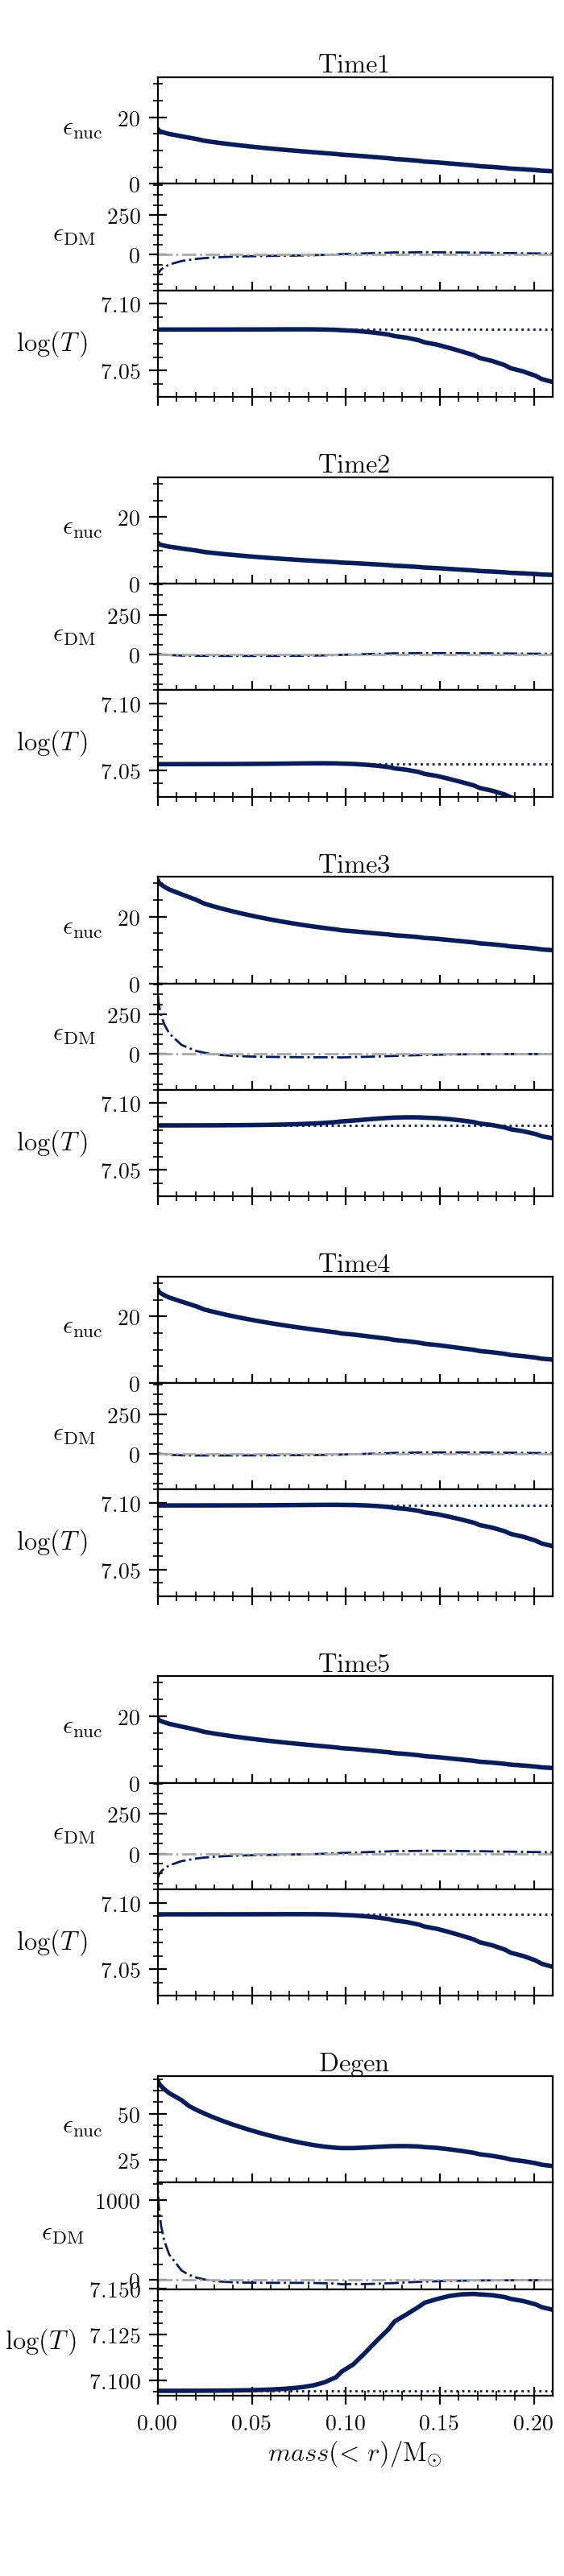
\includegraphics[width=0.47\textwidth]{plots/m1p0c6.png}
    \caption{$1.0 \Msun$ profiles for \nodm (grey) and $\gbpow{6}$ (dark blue) models. In each set of 3 panels, the top 2 are the same as in Figure~\ref{fig:m3p5}. The third panel is the temperature in [K], with the characteristic ADM temperature, $\Tx$, shown as a thin dotted line. ADM energy transport decreases hydrogen burning in the core and pushes the burning into a shell more quickly than the reference models. The reduced central burning causes the $\gbpow{3}$ model to live slightly longer than the \nodm model.
    }
    \label{fig:m1p0c6}
  \end{figure}


Standard model stars in this mass range have relatively low central temperatures and so are powered primarily by the pp chain, which is much less sensitive to the temperature than burning via the CNO cycle. This means the burning does not peak as strongly at the center and radiative transport is sufficient to carry the energy flux, so the core is radiative. Without the mixing provided by convection, hydrogen depletes first at the very center and the burning shifts gradually outward into a shell.

As seen in Fig.~\ref{fig:m1p0c6}, energy transport by large amounts of ADM cause flatter temperature profiles than those seen in the \nodm model. This reduces the burning rate in the center (where ADM is removing energy) and increases it in a shell (where ADM deposits energy).


% fe low mass

% fs high mass
\subsection{High-Mass Stars: \mrangehigh}
\label{sub:highmass}

  % 3.5Msun, energy and convection
  \begin{figure}
    \centering
    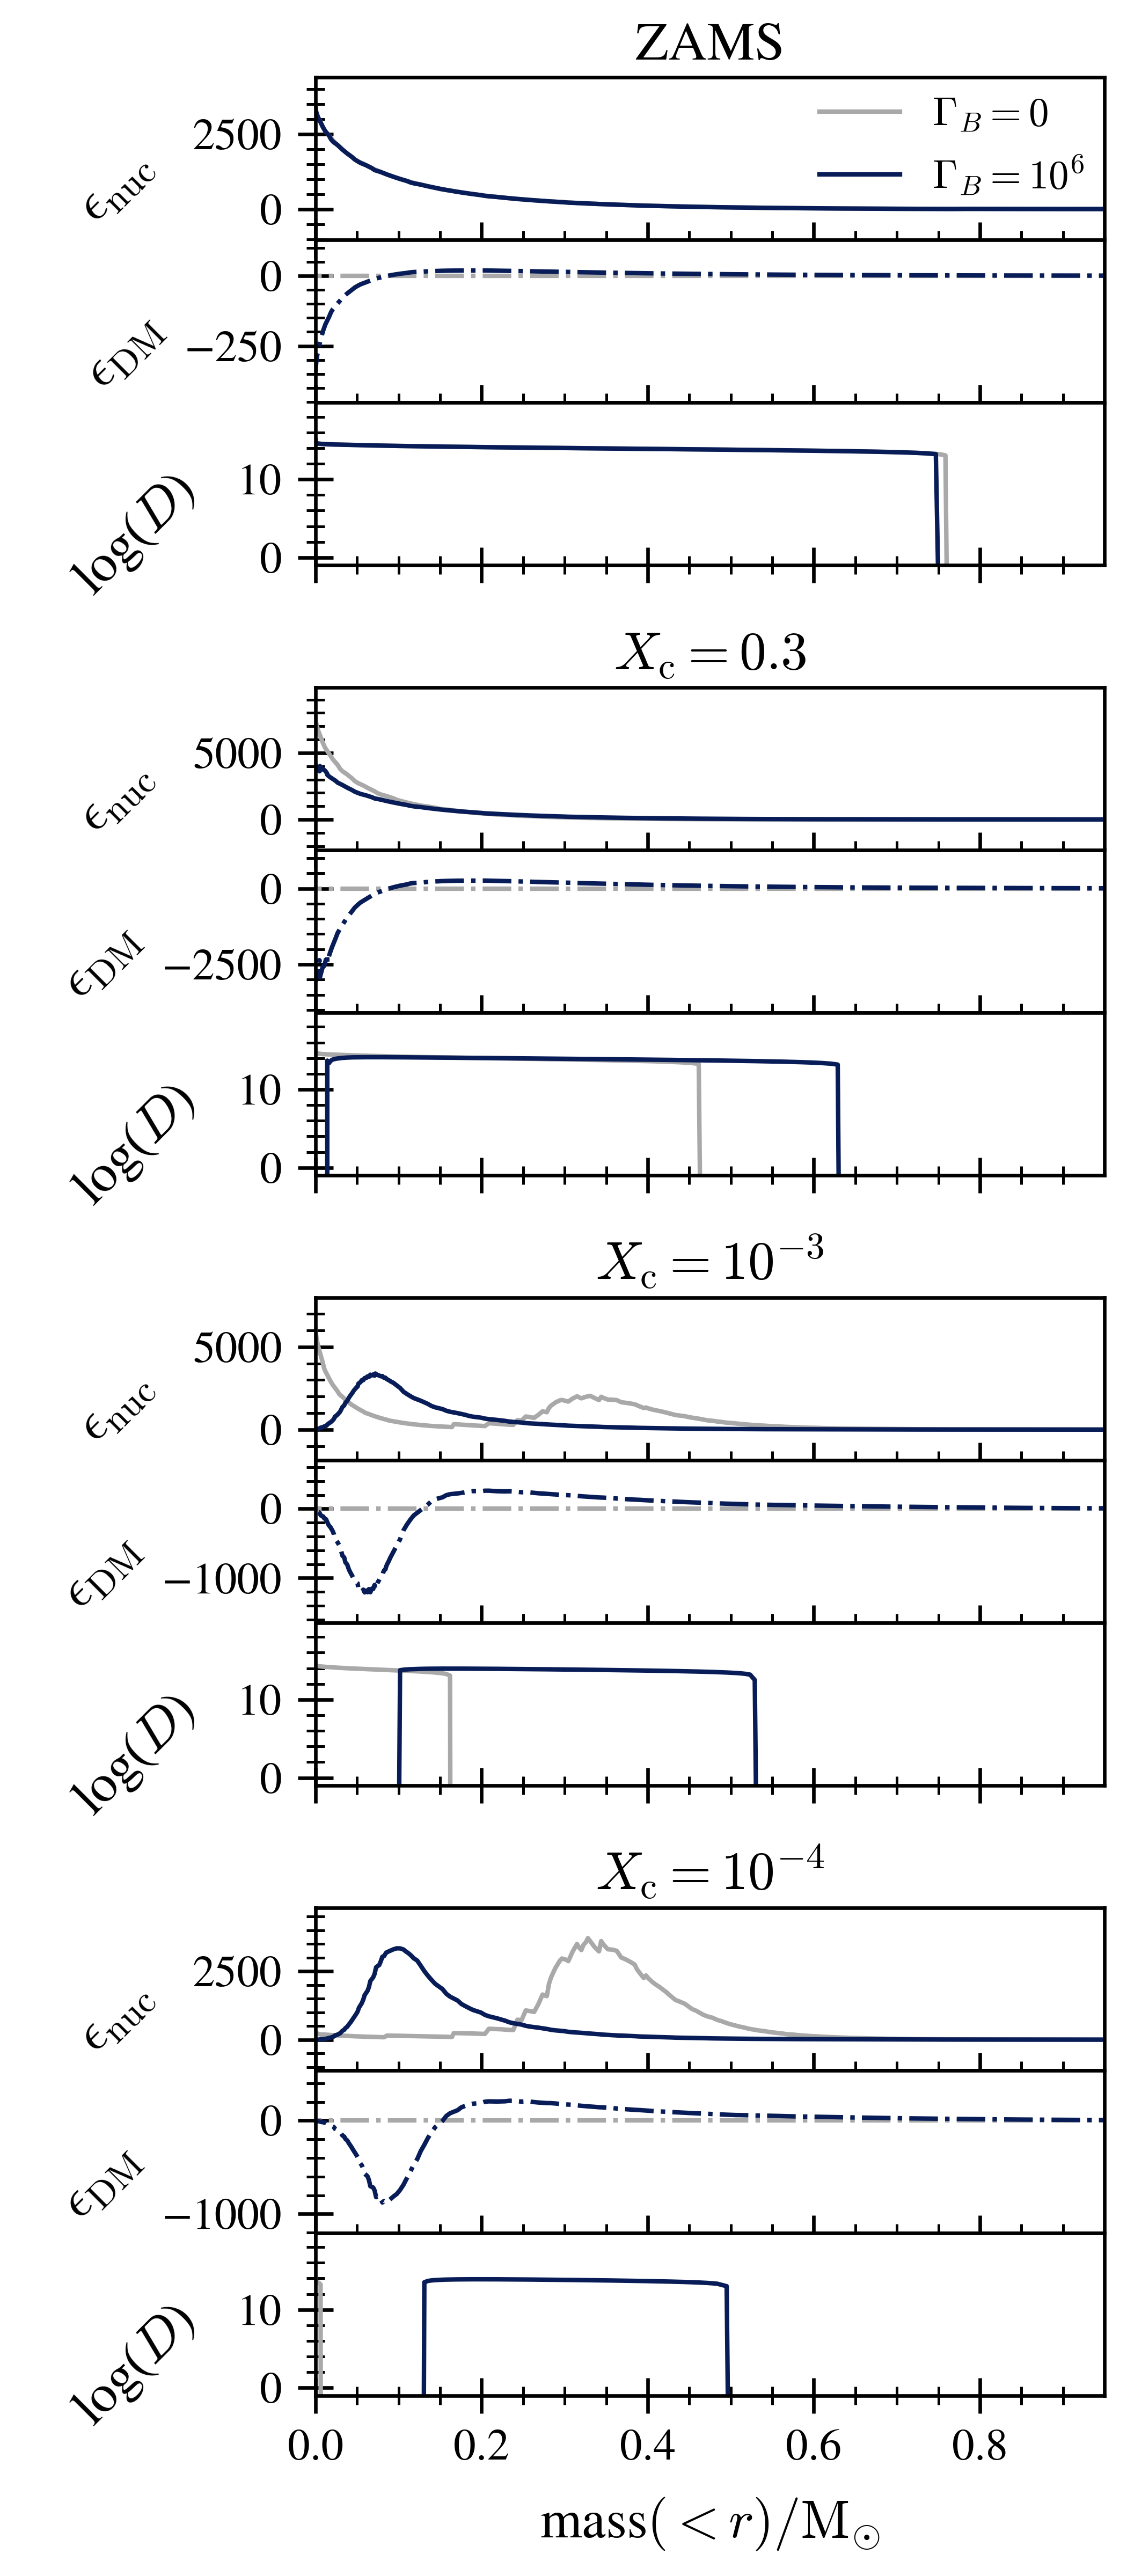
\includegraphics[width=0.47\textwidth]{plots/m3p5.png}
    \caption{$3.5 \Msun$ profiles for \nodm (grey) and $\gbpow{6}$ (dark blue) models. Each set of 3 panels shows stellar profiles of the stars at different evolutionary phases indicated by the fraction of hydrogen in the center, $X_c$, which decreases as the star evolves. The profiles in each panel are: 1) $\epsnuc$, the nuclear burning rate in [erg/g/s], 2) $\epsdm$, the rate at which DM transports energy (negative values indicate that energy is being removed), also in [erg/g/s], 3) D, the diffusion coefficient for convective + overshoot mixing in [cm$^2$/s]. In the \nodm model the convective core shrinks toward the center over time, and the burning rate peaks at the center until the end of the main sequence when the central burning rate drops dramatically and a shell of strong burning appears suddenly. In the $\gbpow{6}$ model, convection at the very center shuts off early in the MS and a convective shell retreats away from the center over time. The peak burning rate shifts gradually outward, following the inner edge of the convective shell.
    }
    \label{fig:m3p5}
  \end{figure}

In standard models, MS stars with $\Mstar \gtrsim 1.3 \Msun$ are powered primarily by the CNO cycle.
This has several important consequences:
(1) the burning rate is much higher than in pp-dominated stars;
(2) the burning rate is extremely sensitive to core temperature;
and (3) stellar cores must be convective in order to carry away the energy produced by core hydrogen burning.
Once hydrogen throughout the convective zone is depleted, the burning rate rapidly decreases, and the star loses more energy at its surface than is being generated by burning. Gravity temporarily dominates over the pressure support from burning and the star contracts until the internal temperature increase is sufficient to ignite hydrogen in a shell outside the depleted core. See Figure~\ref{fig:m3p5}.

If a star captures enough ADM, the combination of dark matter + radiative energy transport becomes sufficient to carry the flux from nuclear burning. Convection disappears from the center first (where ADM energy transport is most efficient) and retreats away from the core, into a narrowing shell. Without convective mixing, the central hydrogen supply depletes first at the very center (instead of simultaneously throughout the core) and the burning also shifts into a shell, following the lower boundary of the convective zone. This can be seen in the time progression (down the page) of the $\gbpow{6}$ (dark blue) model in Figure~\ref{fig:m3p5}. The shift to shell burning is more similar to the behavior of standard low mass models.

% fe high mass

% fs MS lifetimes
\subsection{Main Sequence Lifetimes}
\label{sub:mstau}

% mstau plot
\begin{figure*}
  \centering
  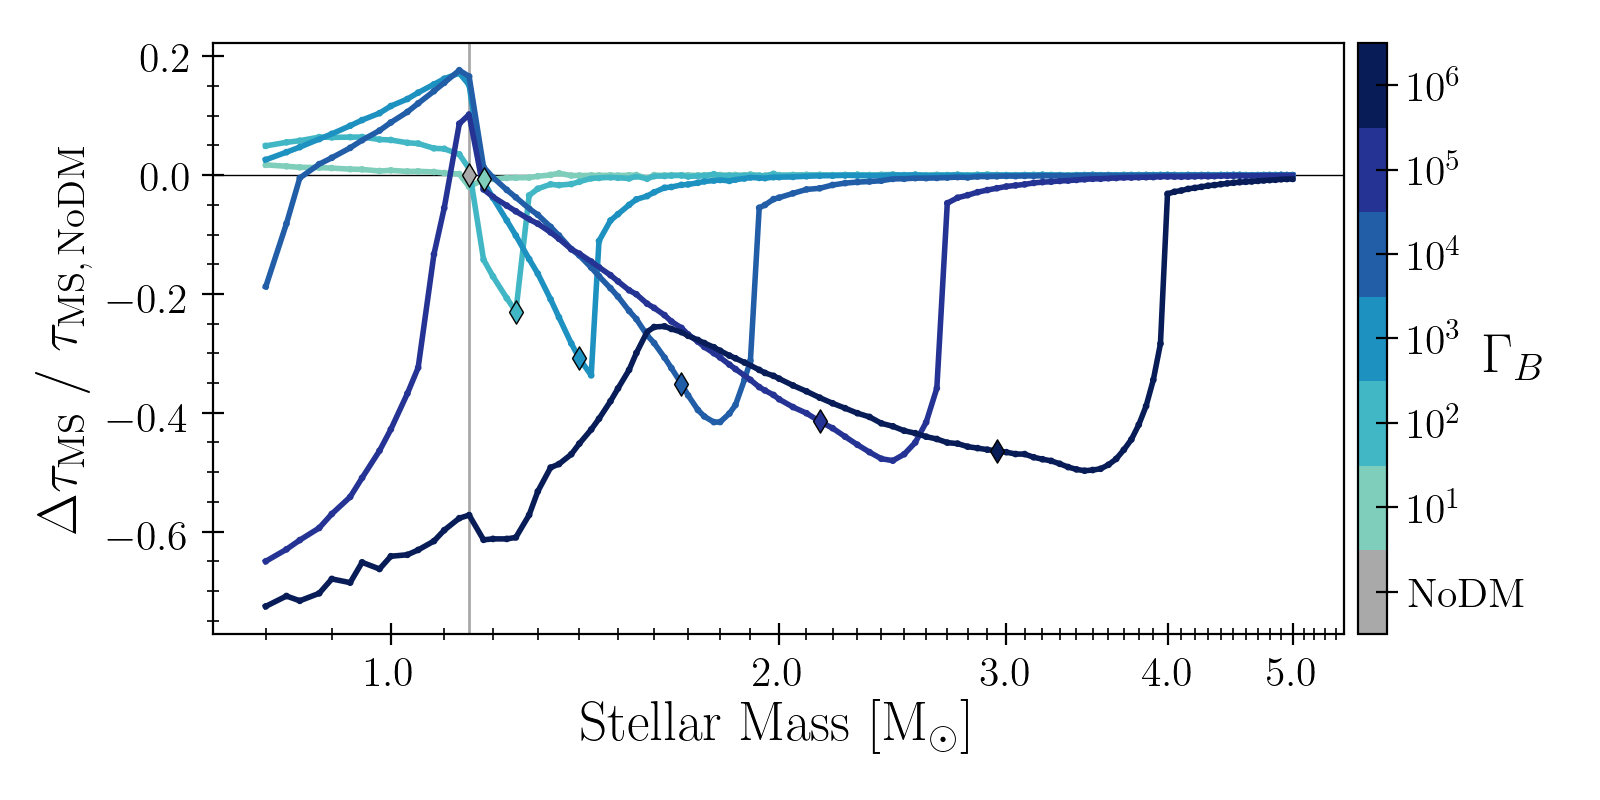
\includegraphics[width=\textwidth]{plots/mstau.png}
  \caption{The presence of ADM tends to shorten MS lifetimes relative to models with no dark matter.
  Diamonds mark the transition from radiative to convective cores (left to right). For the purposes of this figure this is defined as the lowest \Mstar for which the average (over the MS) mass of the convective core is greater than 0.01 Mstar. This transition is also marked by a vertical line for the \nodm model since this is what splits the low and high mass groups. Stars to the right of this line have decreased lifetimes due to a reduction in the size of the convective core, which reduces the amount of hydrogen available for burning. The effect abruptly disappears as stellar lifetimes become shorter than the time required to build up a sufficient amount of ADM. Stars to the left of the vertical line show mixed behavior. Those with lower $\gb$ have increased lifetimes due to decreased burning rates. Those with high $\gb$ show little change.
  }
  \label{fig:mstau}
\end{figure*}

In Fig.~\ref{fig:mstau} we show the effects of ADM on main sequence (MS) lifetimes relative to a standard \nodm star of the same mass. We have defined the MS to end when the fractional abundance of hydrogen in the center, $X_c$, falls below $10^{-3}$ (check the number, MIST defines TAMS = 10^-12). $X_c$ declines rapidly at the end of the MS, so our results are not strongly affected by the exact choice.

Lifetimes of low mass stars, which have radiative (not convective) cores even in \nodm models, are not greatly affected by ADM. Models with intermediate \gammaB values have their lifetimes extended by up to $~20\%$ because the DM energy transport reduces the temperature in the center, which in turn reduces the burning rate. Models that capture large amounts of ADM (high \gammaB values) have very little change in their MS lifetimes. (why? Perhaps the burning rate in the shell is high enough, and the settling happens fast enough that helium ash accumulates in the core at the same rate as in no DM models?)

ADM tends to shorten the lifetimes of high mass stars ($\Mstar \gtrsim 1.3 \Msun$), an effect that increases with \gammaB. In \nodm models, the central convection zone extends beyond the burning region, giving the star a source of fresh nuclear fuel as hydrogen from outside of the core is mixed into the center. Since ADM shuts off convection in the center, the star no longer gets this influx of unburnt hydrogen, therefore it has less fuel to burn and so it leaves the MS faster than the \nodm models. Note that the appearance of the convective core shifts to higher masses with increasing \gammaB (diamonds in Fig.~\ref{fig:mstau}) due to larger amounts of ADM which can carry larger energy fluxes. The effects disappear abruptly as $\Mstar$ approaches $5 \Msun$ because stellar lifetimes (which scale as $\Mstar^{-2.5}$ (check exact number)) quickly become too short for a sufficient amount of ADM to build up in the star (recall that the ADM capture rate scales linearly with $\Mstar$).

% fe MS lifetimes

% fs isochrones
\subsection{Stellar Tracks and Isochrones}
\label{sub:isochrones}

% stellar tracks plots
\begin{figure*}
  \centering
  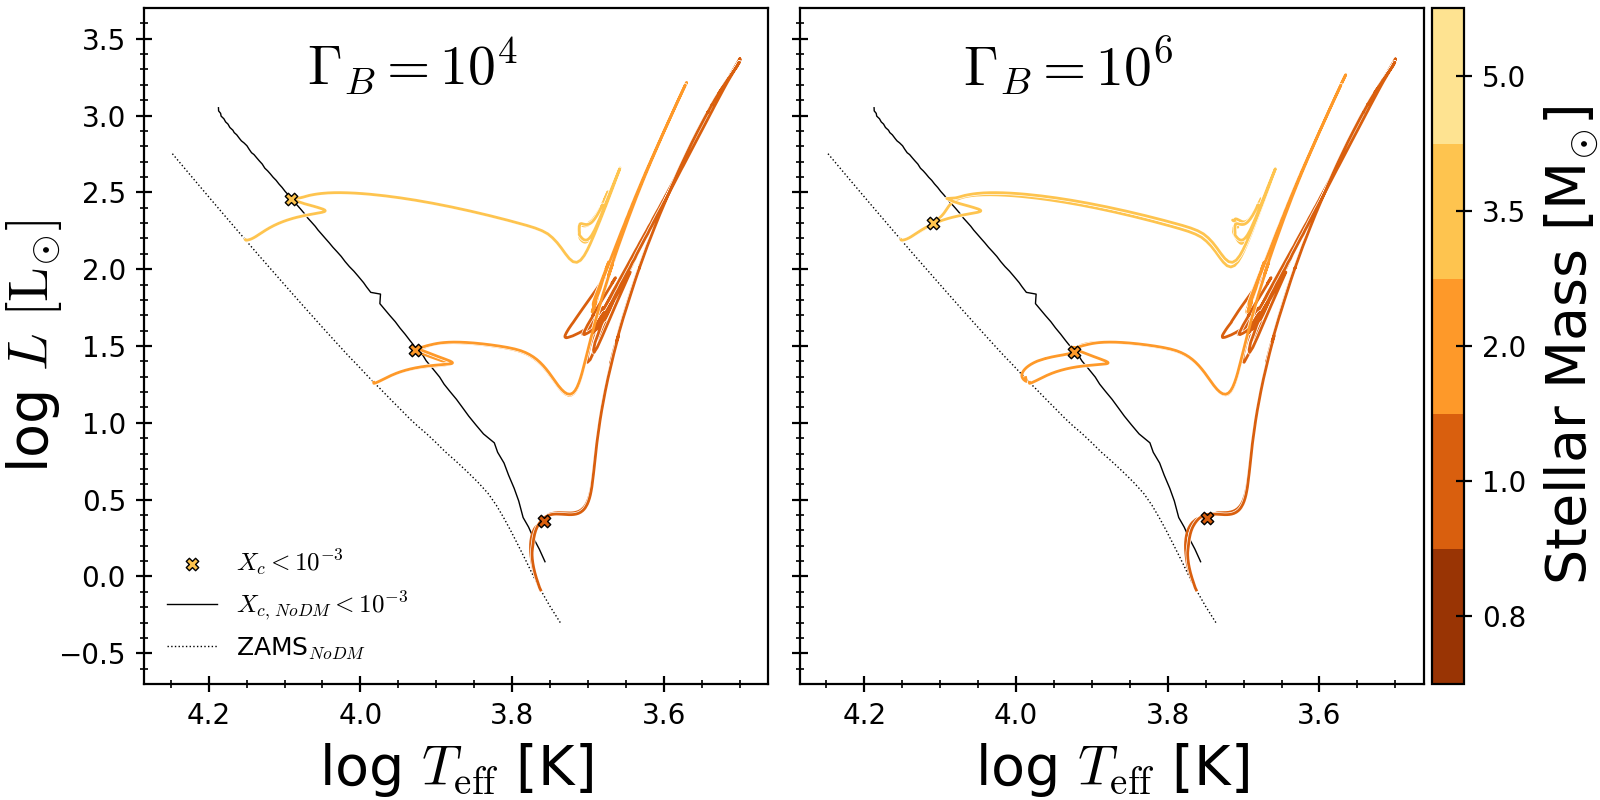
\includegraphics[width=\textwidth]{plots/tracks.png}
  \caption{
  Stellar evolution tracks from ZAMS to core helium depletion ($Y_c<10^{-12}$). x's mark the location where stars leave the MS, defined here as core hydrogen depletion below $X_c<10^{-3}$. The location of the ZAMS and core hydrogen depletion for \nodm models are plotted as dotted and solid black lines respectively. The main effect of ADM on a star's surface properties is to move the star through roughly the same sequence of events at a faster pace, causing the offset of the $X_c<10^{-3}$ milestone relative to \nodm.
  }
  \label{fig:tracks}

\end{figure*}

The HR diagrams in Figure~\ref{fig:tracks} show the effects of ADM on the luminosity and temperature at the stellar surface from the zero age main sequence (“ZAMS”, bottom of each track) through helium core burning. $L$ and $\Teff$ are closely related to the star's magnitude and color which are observable properties. Stars spend most of their time on the MS, burning hydrogen in their cores, and evolve up the track more quickly after leaving the MS.

The effects of ADM on a single star's evolutionary track in an HR diagram (Fig.~\ref{fig:tracks}) are generally subtle since the most significant effect on the surface properties is to move the star through roughly the same sequence of events at a more rapid pace. The location of the ZAMS is set by the balance between pressure support from nuclear burning and gravitational contraction, which depends only on the mass. The temperature of the red giant branch (vertical portion of the tracks) is set by an equilibrium between neutral and ionized hydrogen in the atmosphere. Hence, the star's HR track cannot be too different from the \nodm models.


% isochrones plots
\begin{figure*}
  \centering
  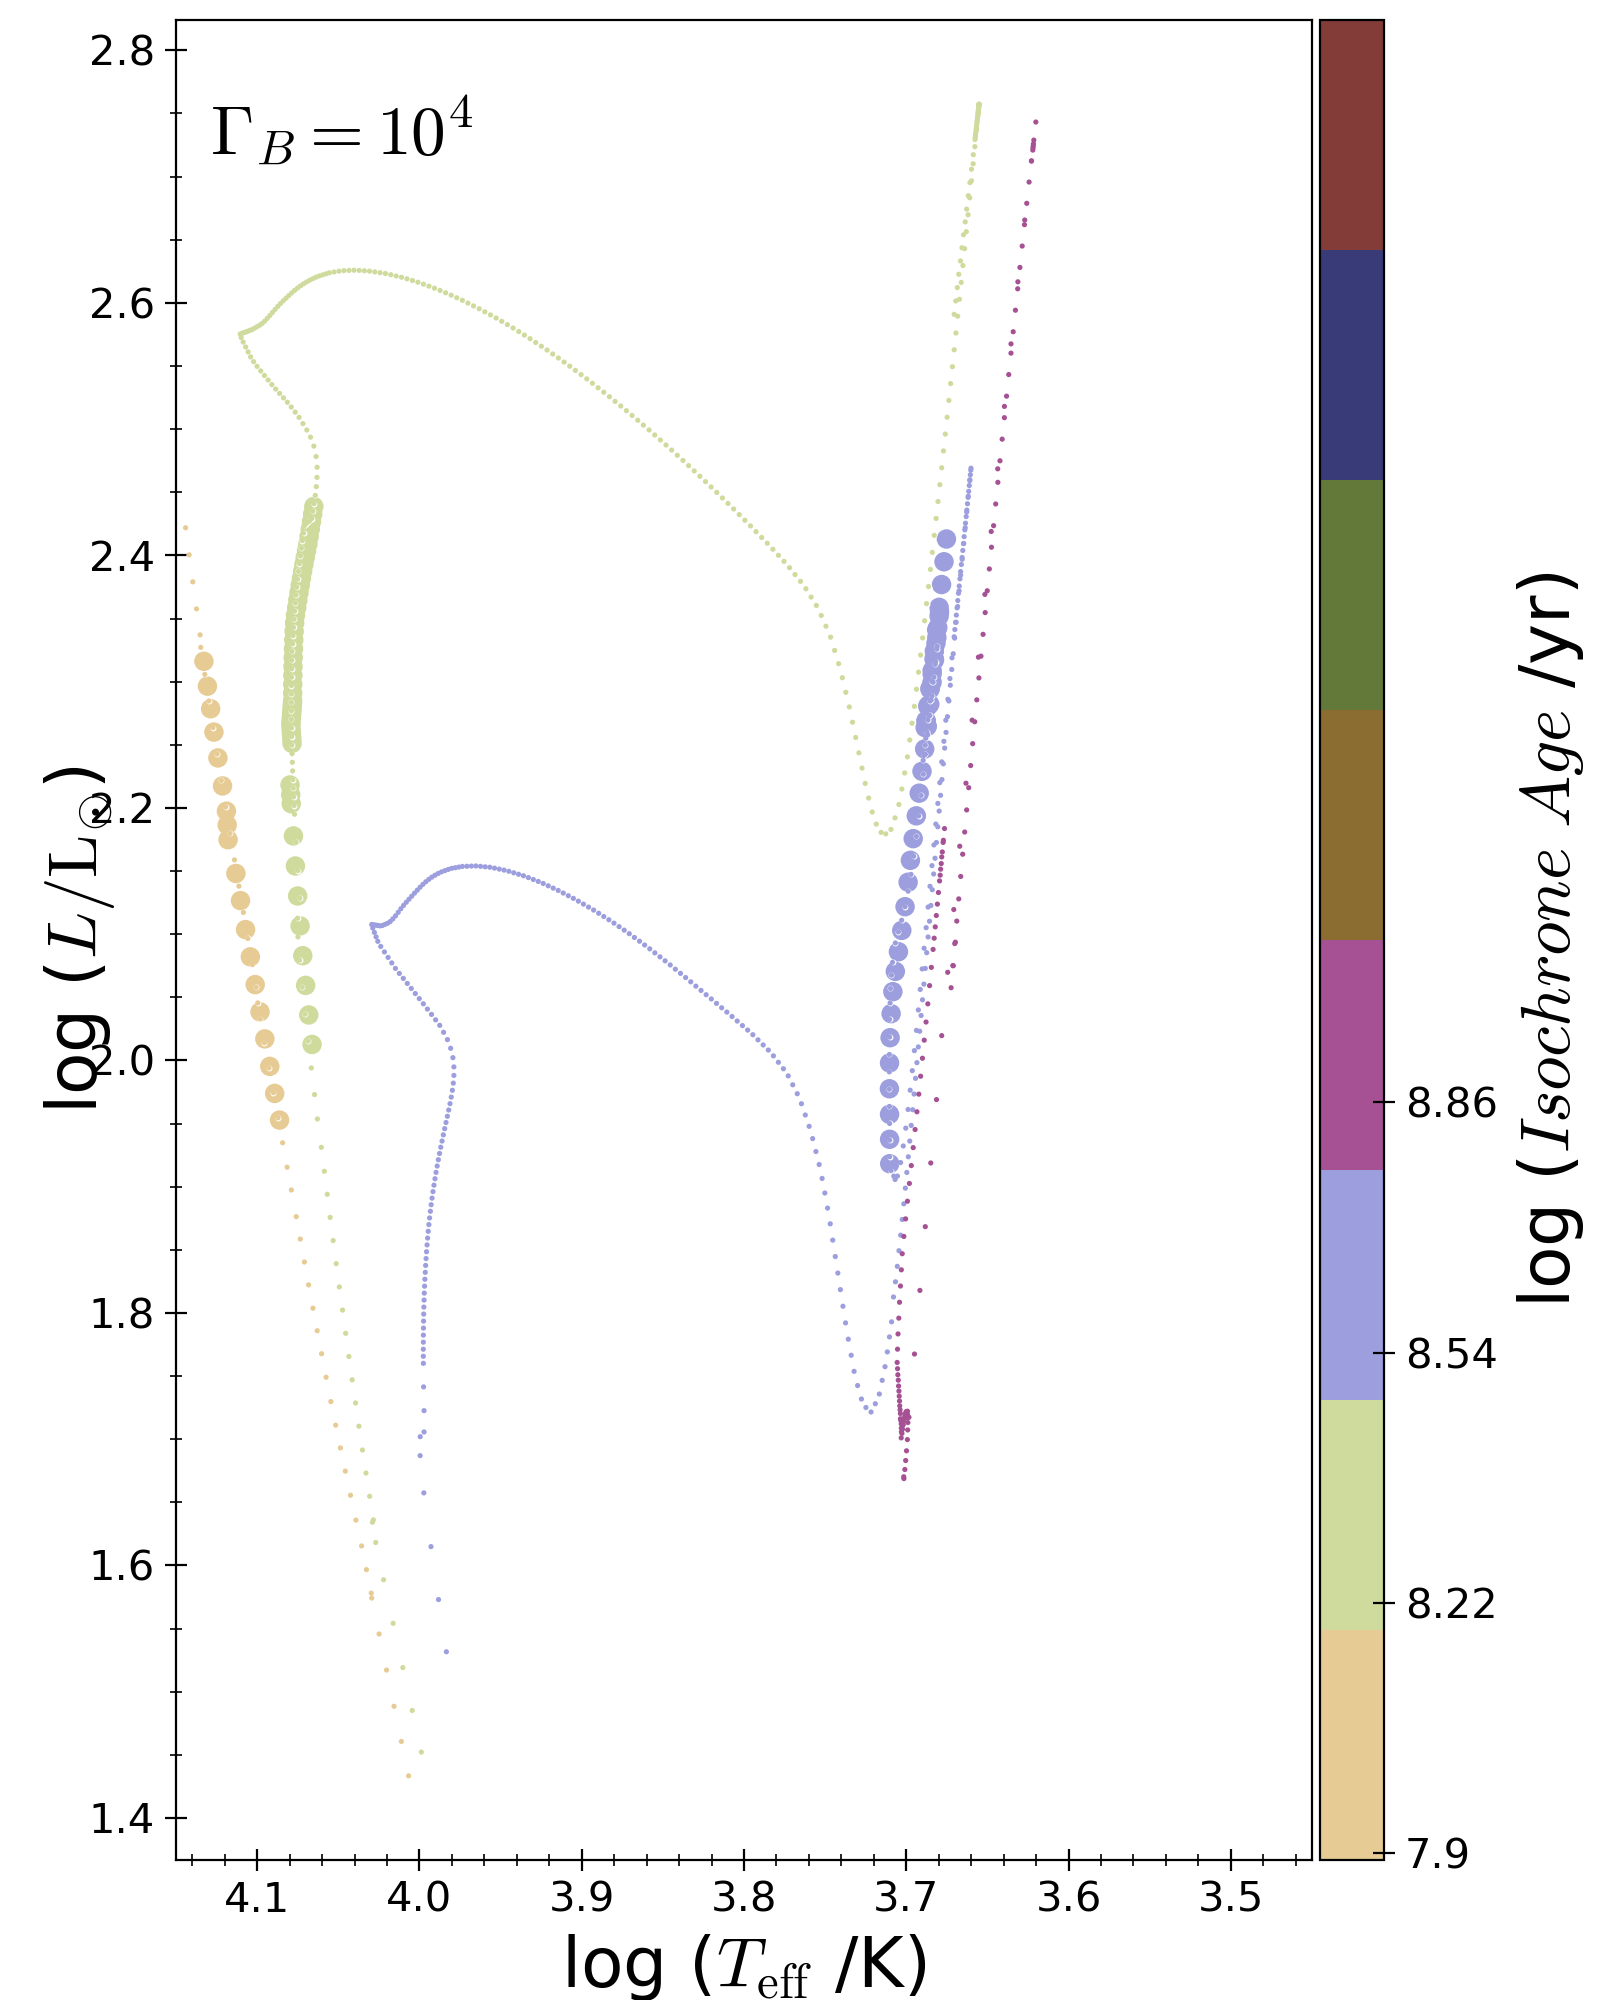
\includegraphics[width=\textwidth]{plots/isos_cb4.png}
  \caption{$\gbpow{4}$ isochrones with \nodm models overplotted as thin lines. Triangles mark $3.5 \Msun$, circles mark $1.0 \Msun$. The positions of the markers here are very similar to the \nodm case (not shown). Gaps in the data are due to the difficulty interpolating in regions where the evolution of lower mass stars is \textit{faster} than that of stars with slightly higher masses (see \S~\ref{sub:isochrones}).
  }
  \label{fig:isos_cb4}
\end{figure*}

\begin{figure*}
  \centering
  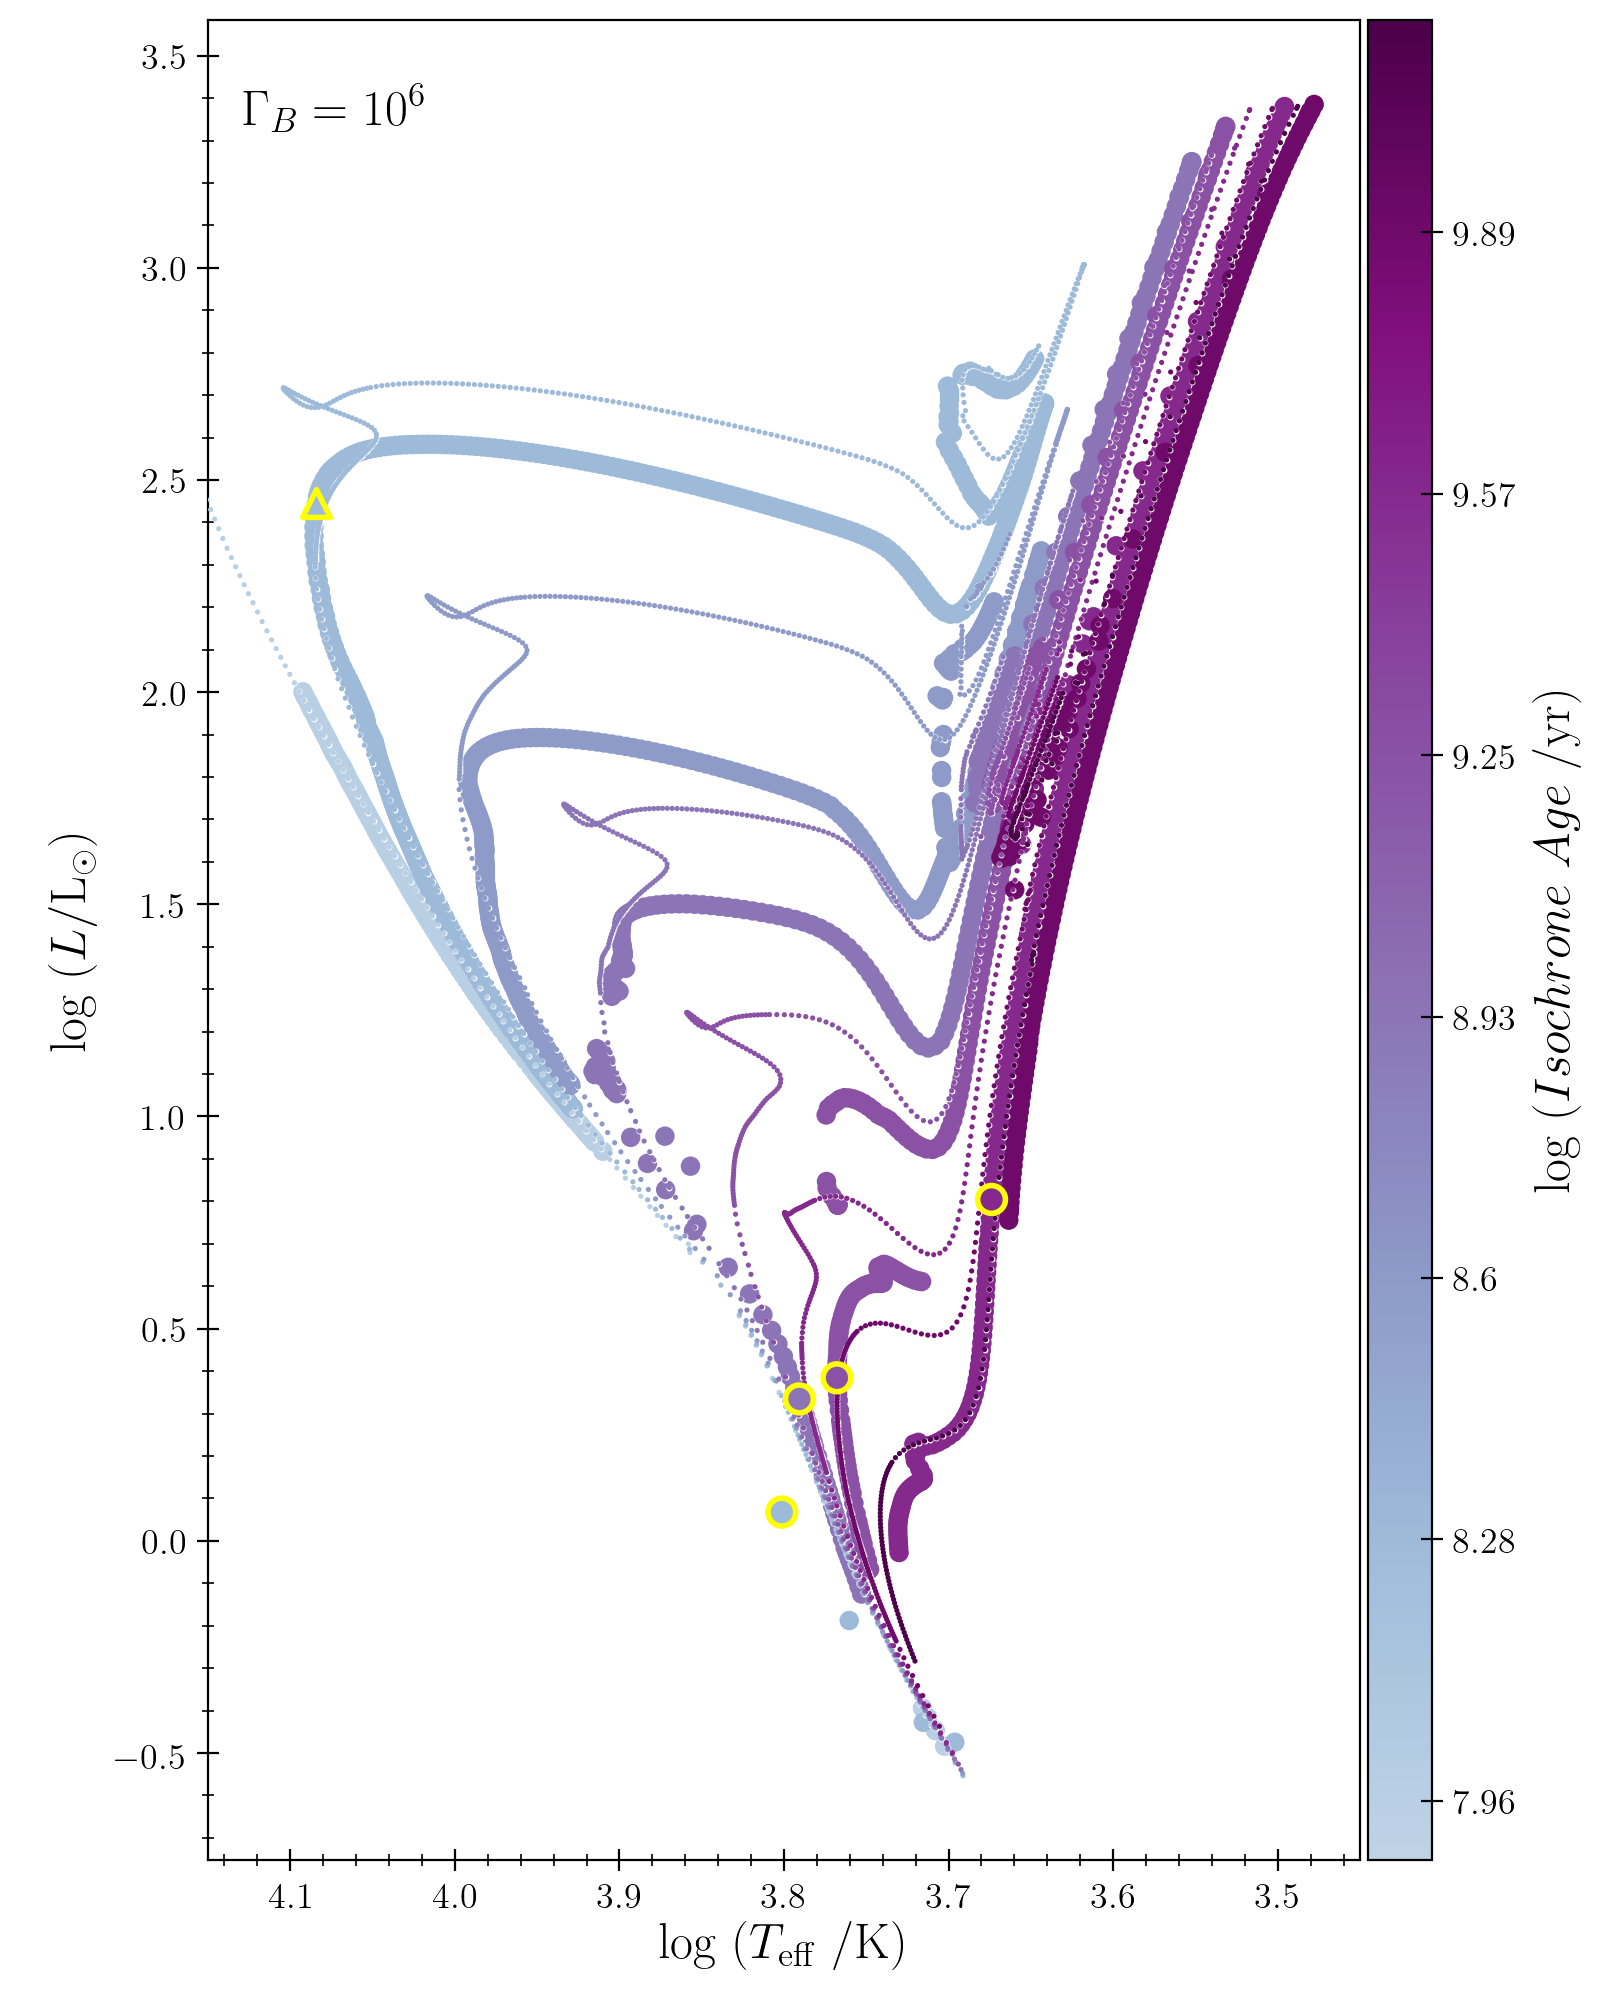
\includegraphics[width=\textwidth]{plots/isos_cb6.png}
  \caption{Same as Fig.~\ref{fig:isos_cb4} but for $\gbpow{6}$. The MS turnoff of isochrones between (insert ages) happens at a lower luminosity and skips the convective hook, causing them to appear older relative to \nodm isochrones.
  }
  \label{fig:isos_cb6}
\end{figure*}


The isochrones in Figures~\ref{fig:isos_cb4} and \ref{fig:isos_cb6} show the effects of ADM on a stellar population. Each isochrone represents a group of stars at a fixed age with a range of masses. Stellar mass increases from bottom to top, and the locations of $1 \Msun$ (circles) and $3.5 \Msun$ (triangles) stars are shown for reference.

The change in MS lifetimes due to ADM is seen here as a shift in the location of the MS turn-off (where the isochrones take a hard right turn, e.g., near the yellow triangle in Figure~\ref{fig:isos_cb6}). Because the general effect on stars that are altered by ADM is to shorten MS lifetimes, the turn-off happens at a lower mass and the stars evolve through the sub-giant branch at a lower luminosity. This causes isochrones of clusters in high $\gb$ environments to appear older than their standard model counterparts. This becomes noticeable in the highest $\gb$ environments around 0.2 Gyr as stars with $\rm{M} \approx 4 \Msun$ begin to leave the MS. Prior to this, the stars have not had enough time to capture a sufficient number of DM particles for ADM-driven energy transport to be a significant contribution to the overall energy transfer within the stars.

Younger \nodm isochrones display a sharp feature called the convective hook near the MS turn-off, which is noticeably absent from the $\gbpow{6}$ isochrones. Since the \nodm models have convective cores, hydrogen is depleted nearly simultaneously throughout the volume of the core at the end of the MS. This causes the burning rate to decrease dramatically, which reduces the pressure support and results in gravitational contraction. The contraction increases the temperature until the bottom layer of hydrogen (now in a shell surrounding the core) is hot enough to ignite, reestablishing the pressure support. Our high $\gb$ isochrones lack this convective hook because ADM shuts off core convection. This lack of mixing causes the hydrogen to deplete first at the very center, and the burning gradually shifts into a shell, avoiding the sudden instability that causes the convective hook. This gradual shift to shell burning is very similar to the low mass \nodm models (which also do not experience a convective hook), which contributes to the high $\gb$ appearing older.

The gaps in the data are due to difficulty interpolating masses at a fixed time. Stellar masses generally increase when following a single isochrone from bottom to top. To build the isochrones from MESA's stellar models, MIST identifies the ages at which each star reaches a series of evolutionary milestones, and interpolates the stellar mass to generate properties of a group of stars at a fixed age. More massive stars generally evolve more quickly, and so the mapping between age and mass at a fixed milestone is usually monotonic, which the interpolation relies on. Exceptions to the monotonicity occur in mass regions where slightly less massive stars evolve more quickly. For example, in \nodm models, the emergence of a convective core around $1.3 \Msun$ results in stars just above this threshold living slightly \textit{longer} than stars just below it. With large amounts of ADM, the increase in stellar lifetimes through this transition to a convective core is much larger than in \nodm models and occurs over a wider mass range. These regions are not interpolated and appear as "missing" data in the isochrones.


% MS turnoff (hottest MS star) Teff and L plots
\begin{figure*}
    \centering
    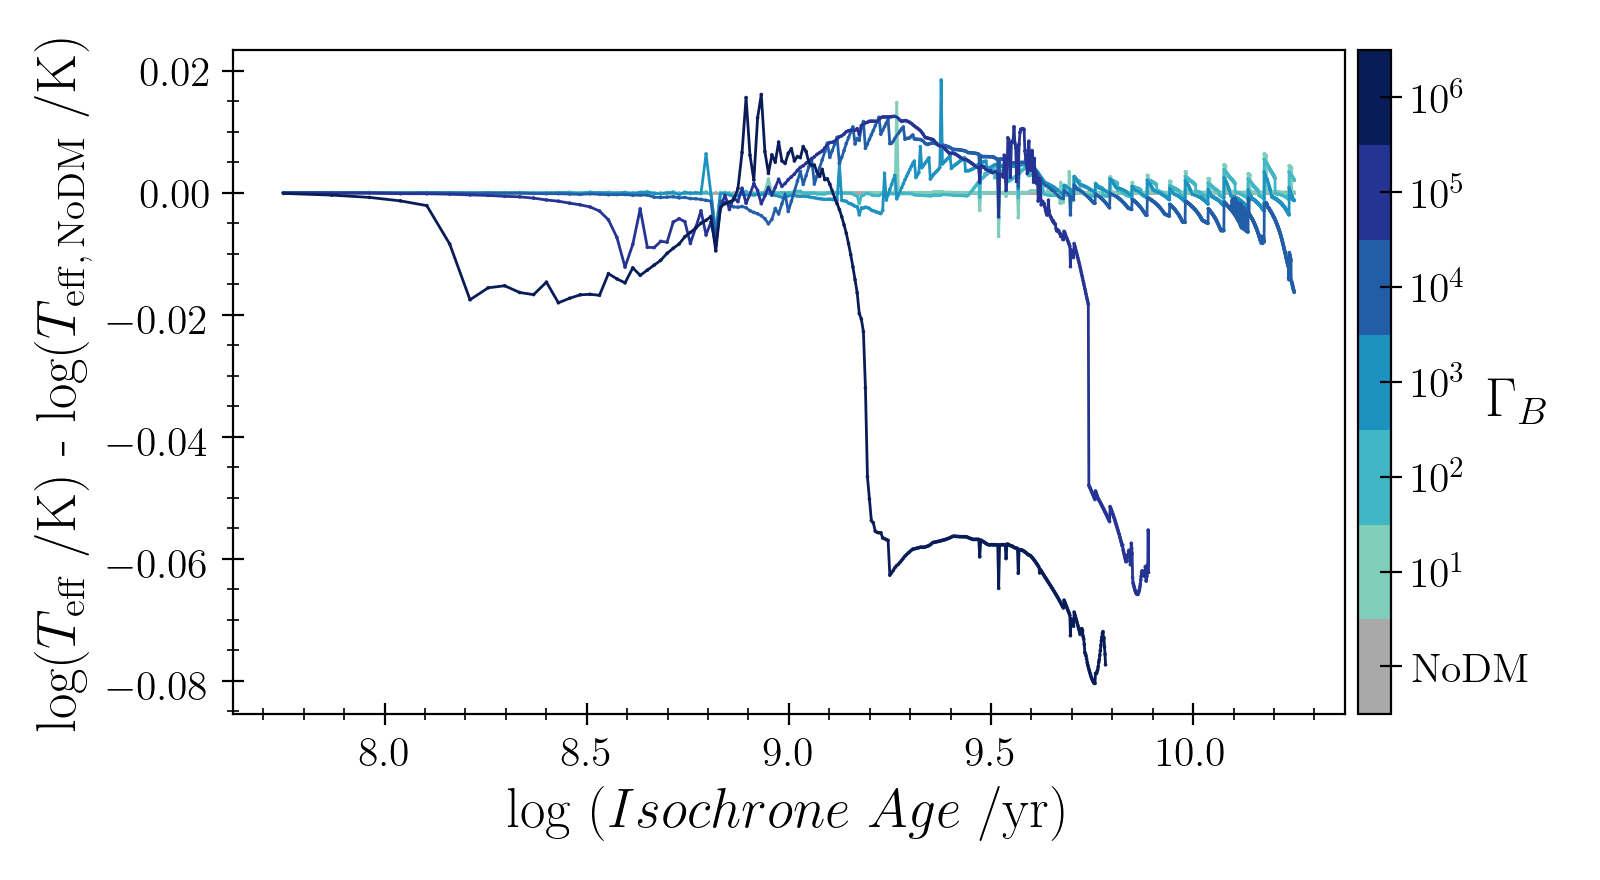
\includegraphics[width=\textwidth]{plots/hotTeff_resid.png}
    \caption{ PLACEHOLDER for MS turn off plots, Teff and/or L.
    Main sequence turnoff temperature (temperature of the hottest star that is still on the main sequence). Residuals are with respect to (...?)
    }
    \label{fig:hotTeff}

\end{figure*}

Paragraph(s) on MS turnoff plots (Teff and/or L as fnc of isochrone age)

% fe isochrones



% fs Pre-Sprint Results Section
\section{Results}
\label{sec:results}

  % mstau plot
  \begin{figure*}
    \centering
    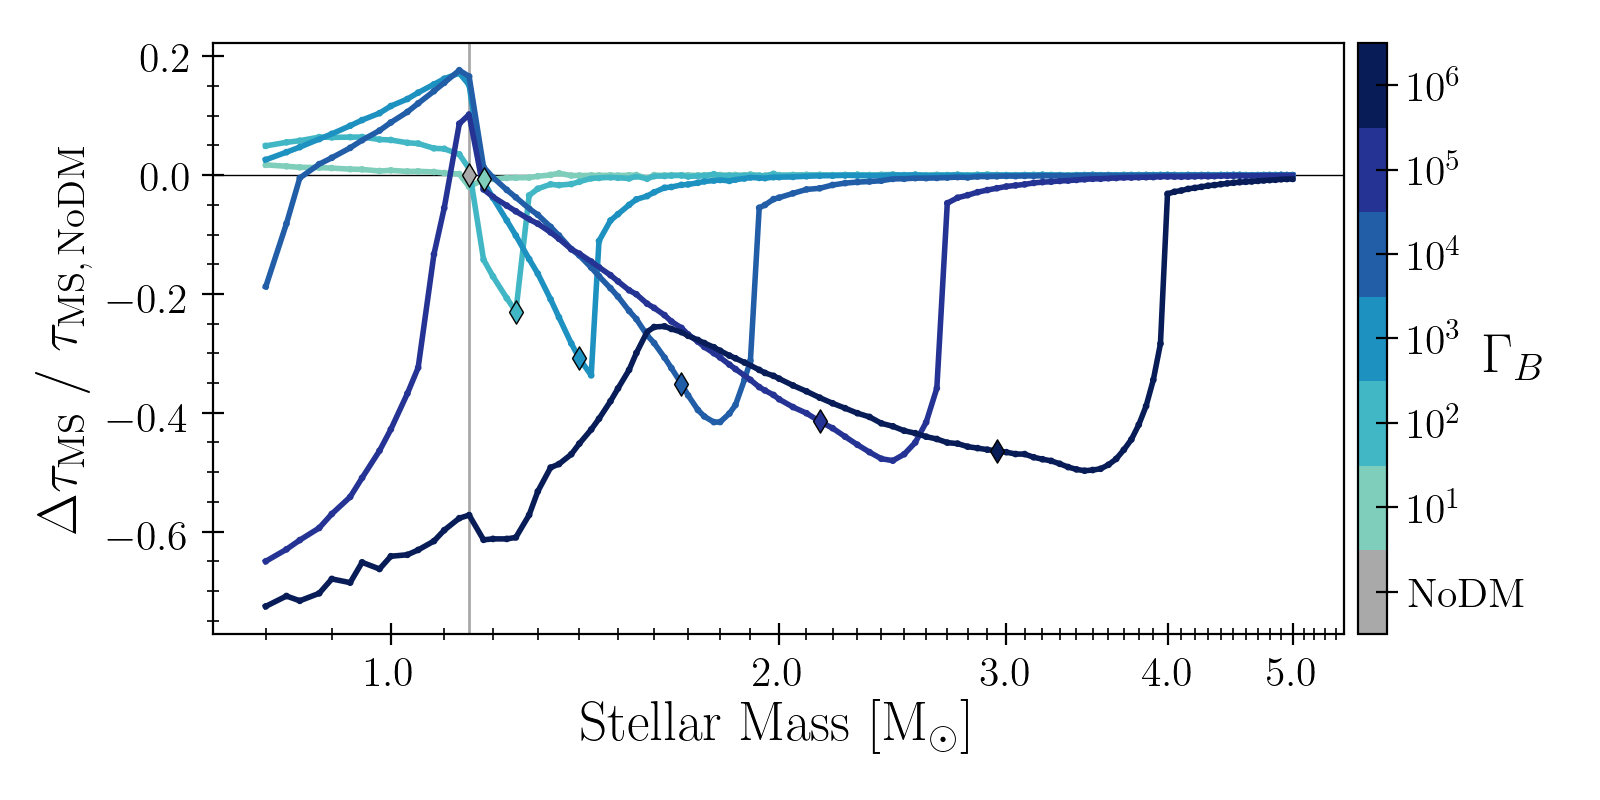
\includegraphics[width=\textwidth]{plots/mstau.png}
    \caption{The presence of ADM tends to shorten MS lifetimes relative to models with no dark matter.
    % Change in MS lifetimes relative to standard model stars with no ADM.
    Diamonds mark the transition from radiative to convective cores (left to right). This transition is also marked by a vertical line for the \nodm model. Stars to the right of this line have decreased lifetimes due to a reduction in the size of the convective core, which reduces the amount of hydrogen available for burning. The effect abruptly disappears as stellar lifetimes become shorter than the time required to build up a sufficient amount of ADM. Stars to the left show mixed behavior. Those with lower $\gb$ have increased lifetimes due to decreased burning rates. Those with high $\gb$ become unstable with extended periods of high burning rates which cause decreased lifetimes. \tjr{to text->} cc transition defined as the lowest mass for which the mass of the cc core (averaged over the MS lifetime) > 0.01 Mstar.
    }
    \label{fig:mstau}
  \end{figure*}

  % Teff plot
  \begin{figure*}
    \centering
    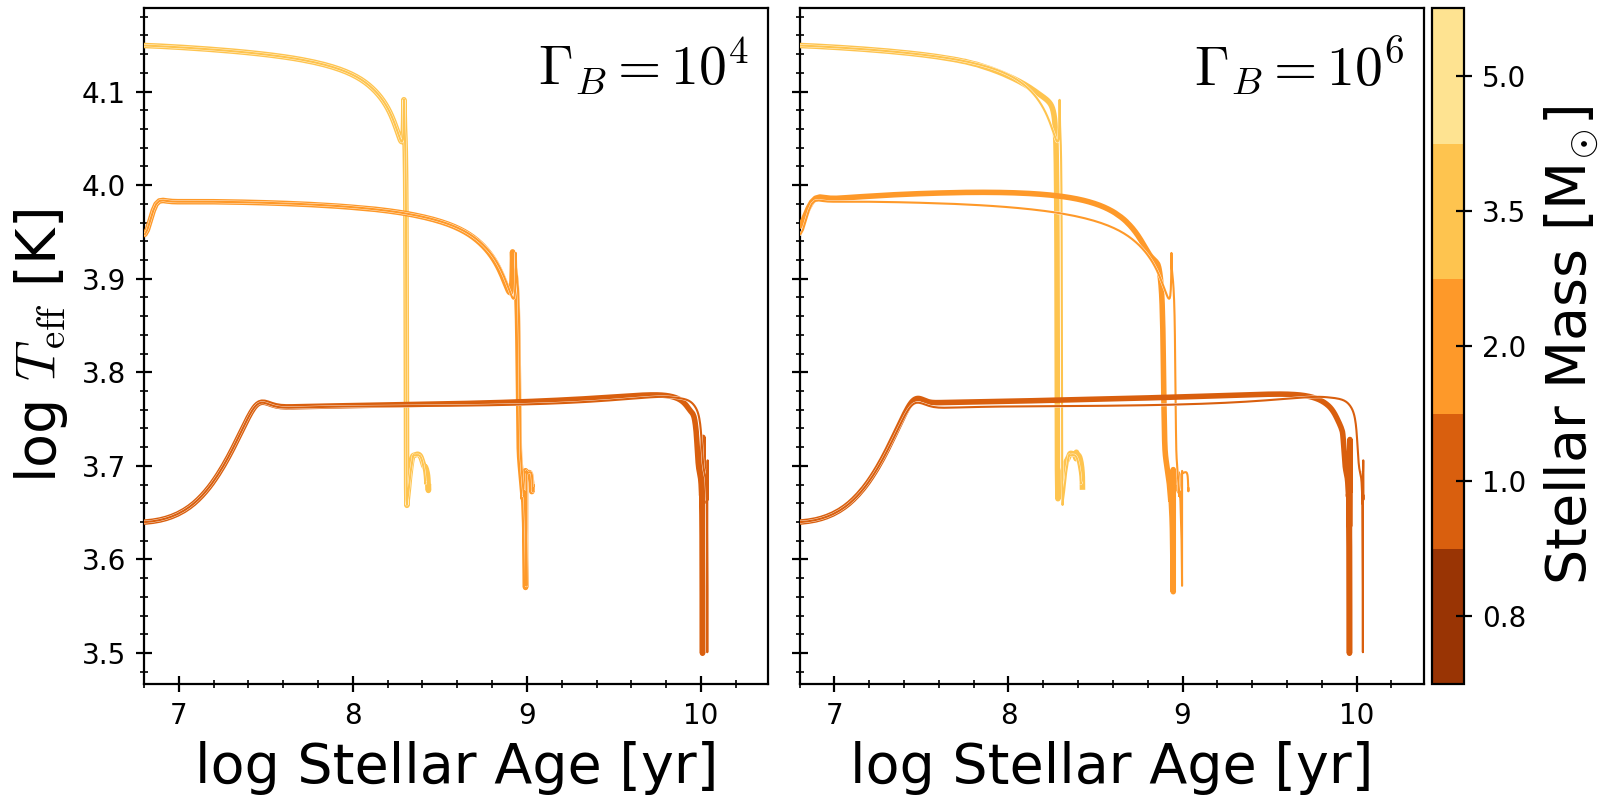
\includegraphics[width=\textwidth]{plots/Teff.png}
    \caption{$\Teff$ as a function of age for select $\gb$, with \nodm models overplotted as thin lines. Stars undergo a sharp decrease in $\Teff$ as they leave the MS. The change in MS lifetimes due to ADM can be seen in the time difference between these features. The surface effects of core oscillations discussed in \S~\ref{sub:lowmass} can be seen here in $\Teff$.
    }
    \label{fig:Teff}
  \end{figure*}

  % stellar tracks plots
  \begin{figure*}
    \centering
    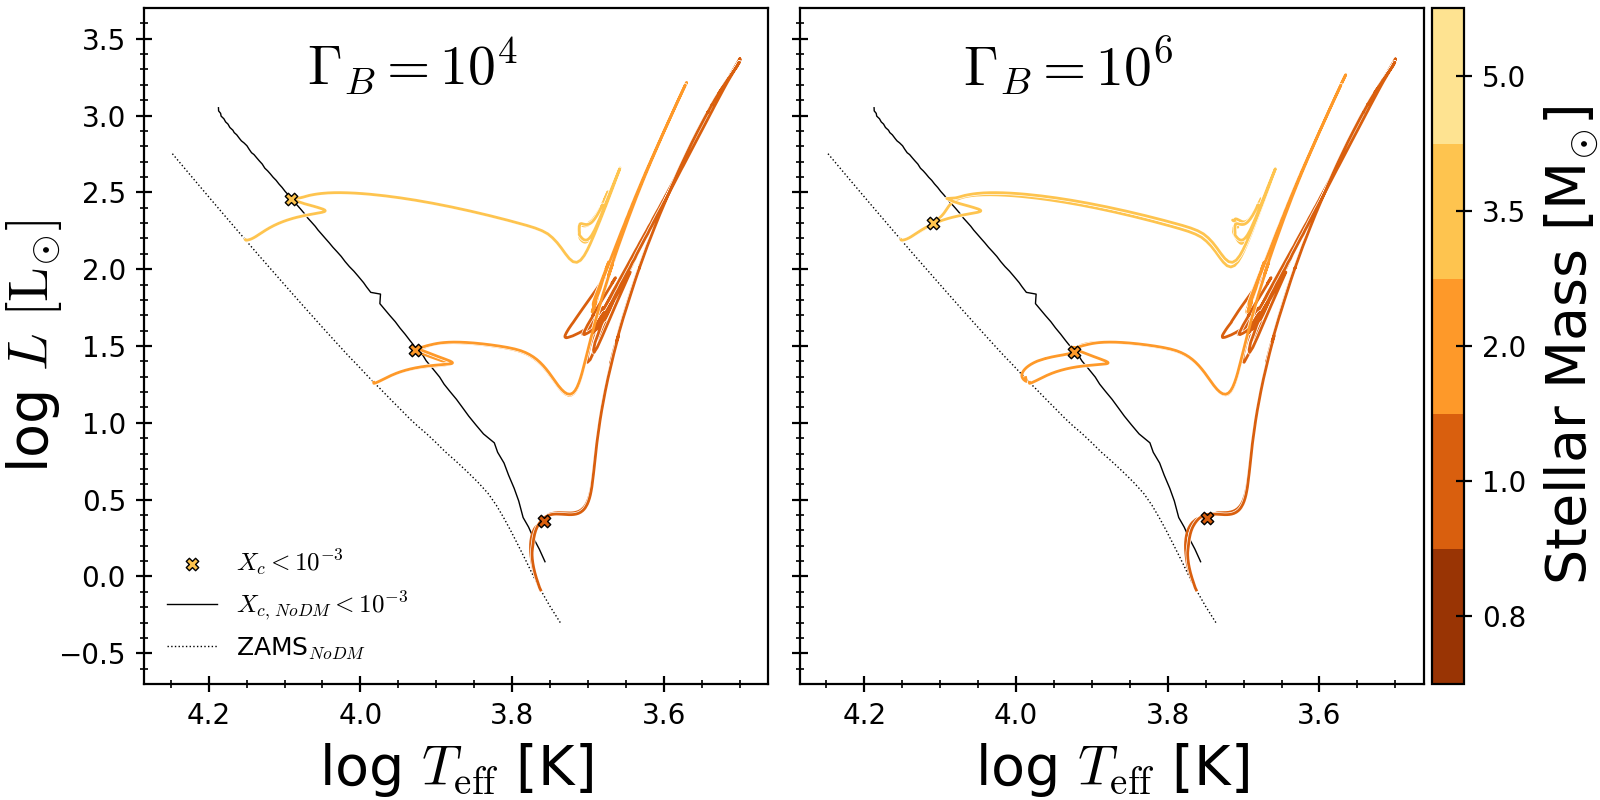
\includegraphics[width=\textwidth]{plots/tracks.png}
    \caption{
    Stellar evolution tracks from ZAMS to core helium depletion ($Y_c<10^{-12}$). x's mark the location where stars leave the MS, defined here as core hydrogen depletion below $X_c<10^{-3}$. For reference, the location of the ZAMS and core hydrogen depletion for \nodm models are plotted as dotted and solid black lines respectively.
    }
    \label{fig:tracks}

  \end{figure*}

  % isochrones plots
  \begin{figure*}
    \centering
    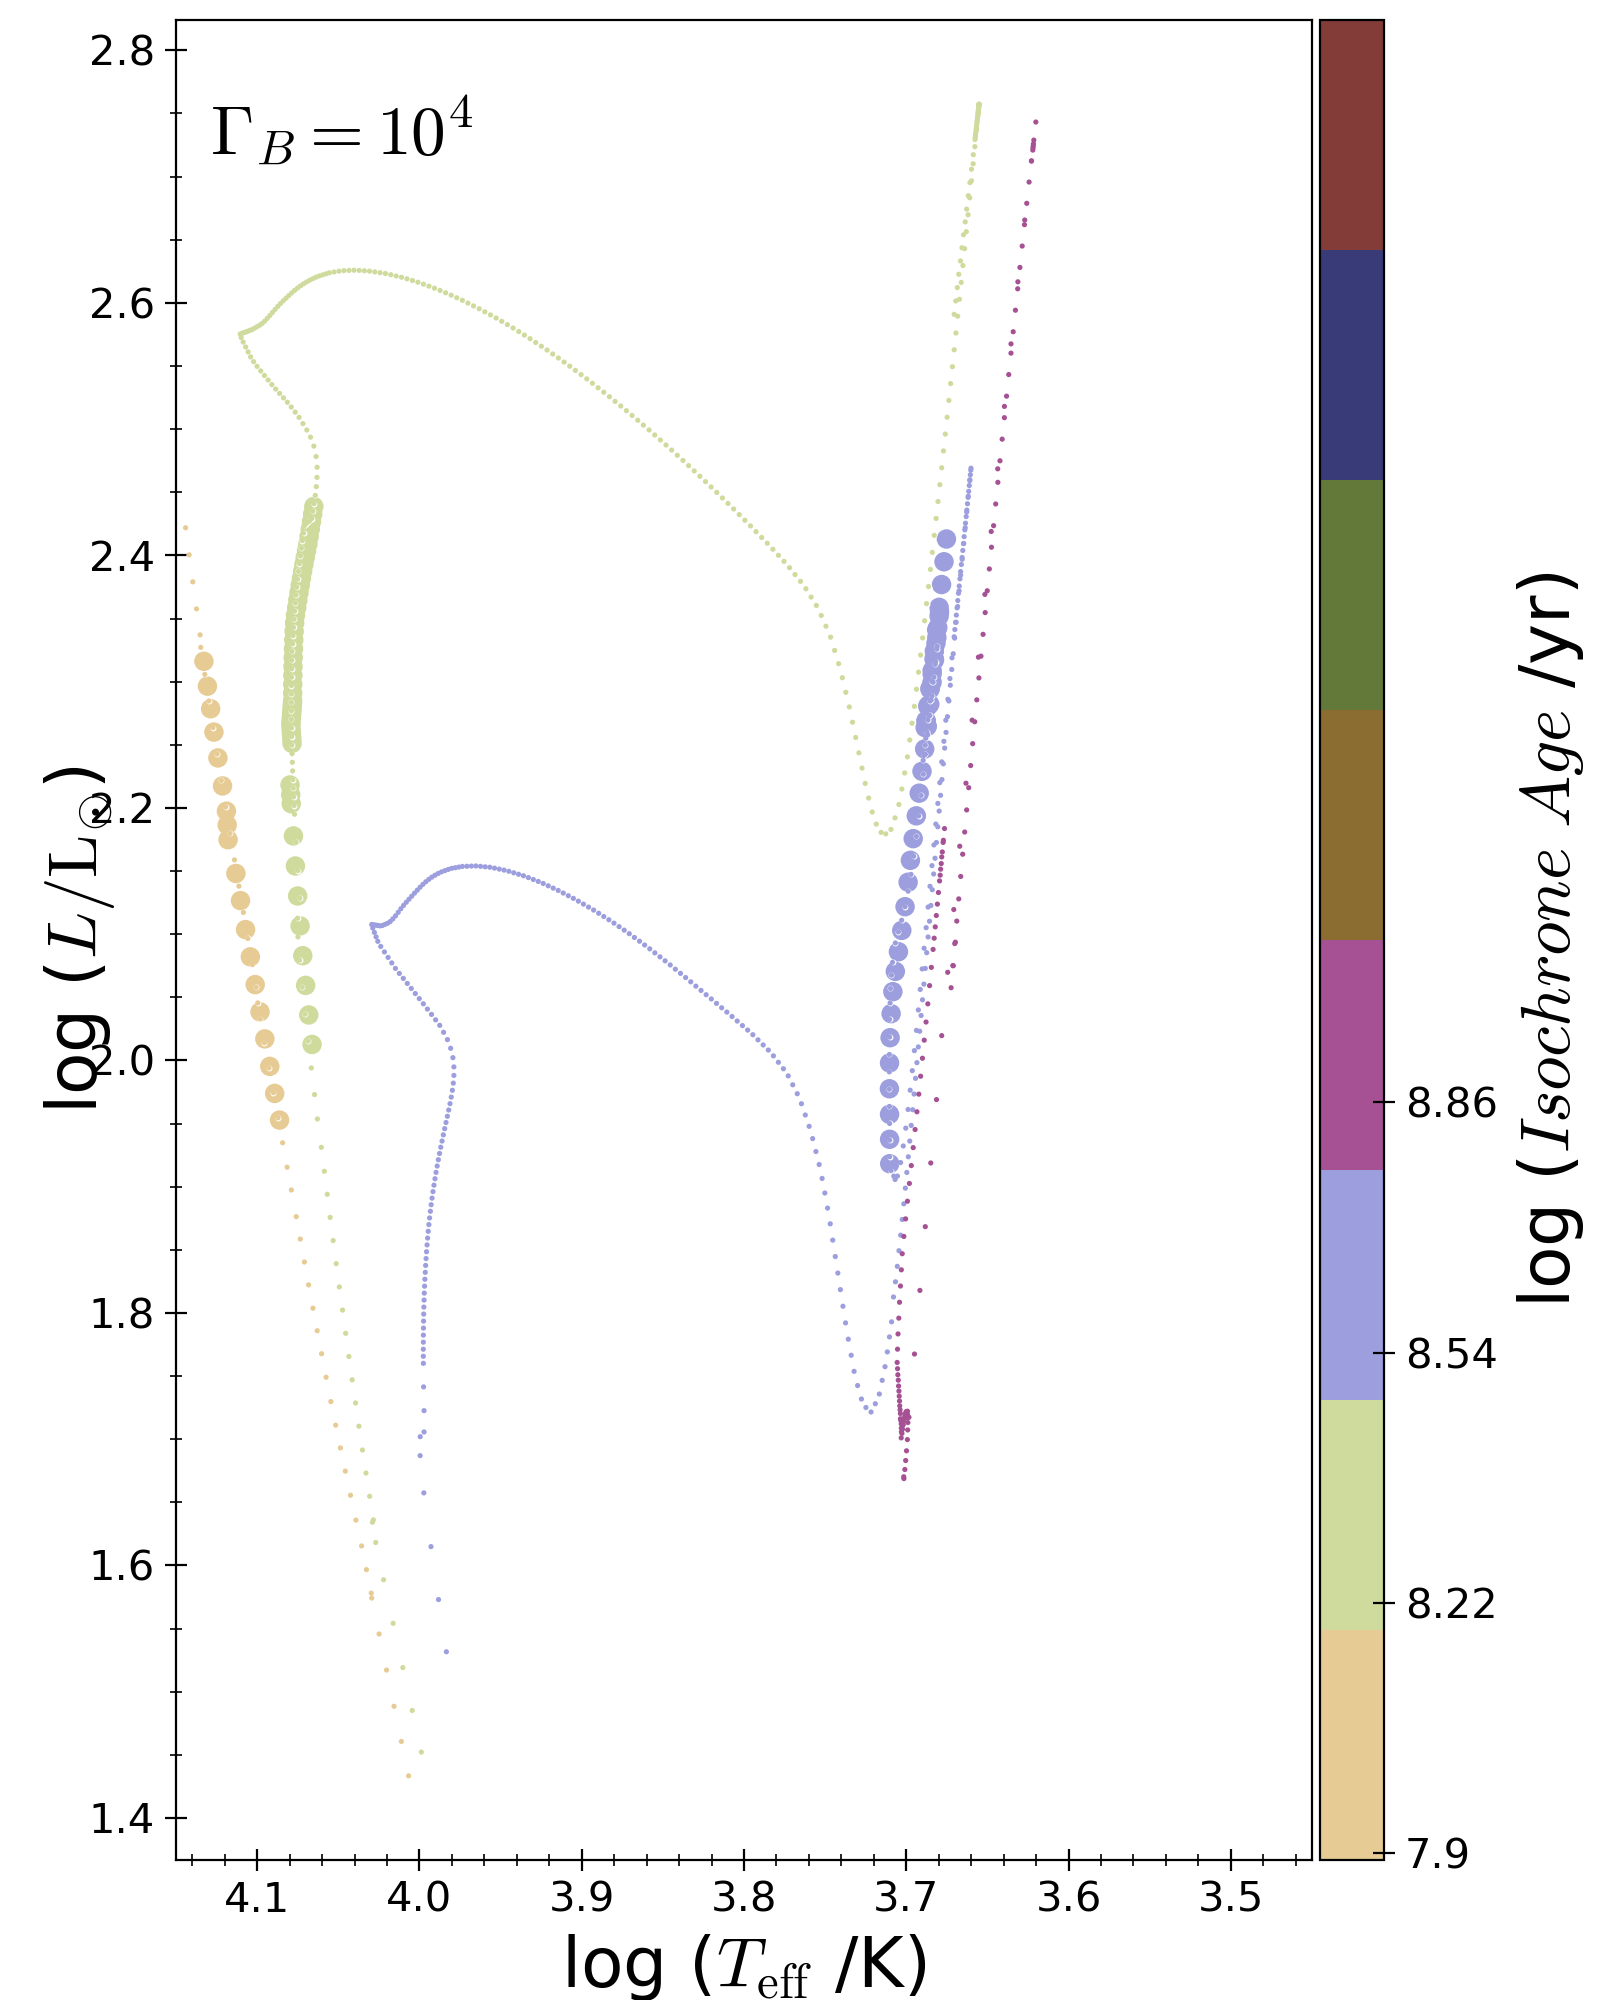
\includegraphics[width=\textwidth]{plots/isos_cb4.png}
    \caption{$\gbpow{4}$ isochrones with \nodm models overplotted as thin lines. Triangles mark $3.5 \Msun$, circles mark $1.0 \Msun$. The positions of the markers here are very similar to the \nodm case (not shown). Gaps in the data are due to the difficulty interpolating in regions where the stellar mass - age relation of a given EEP (equivalent evolutionary phase) is non-monotonic. This is a known problem that Dotter discusses in his paper. \tjr{these last two sentences need work (and need to be mentioned in the text).}}
    \label{fig:isos_cb4}
  \end{figure*}

  \begin{figure*}
    \centering
    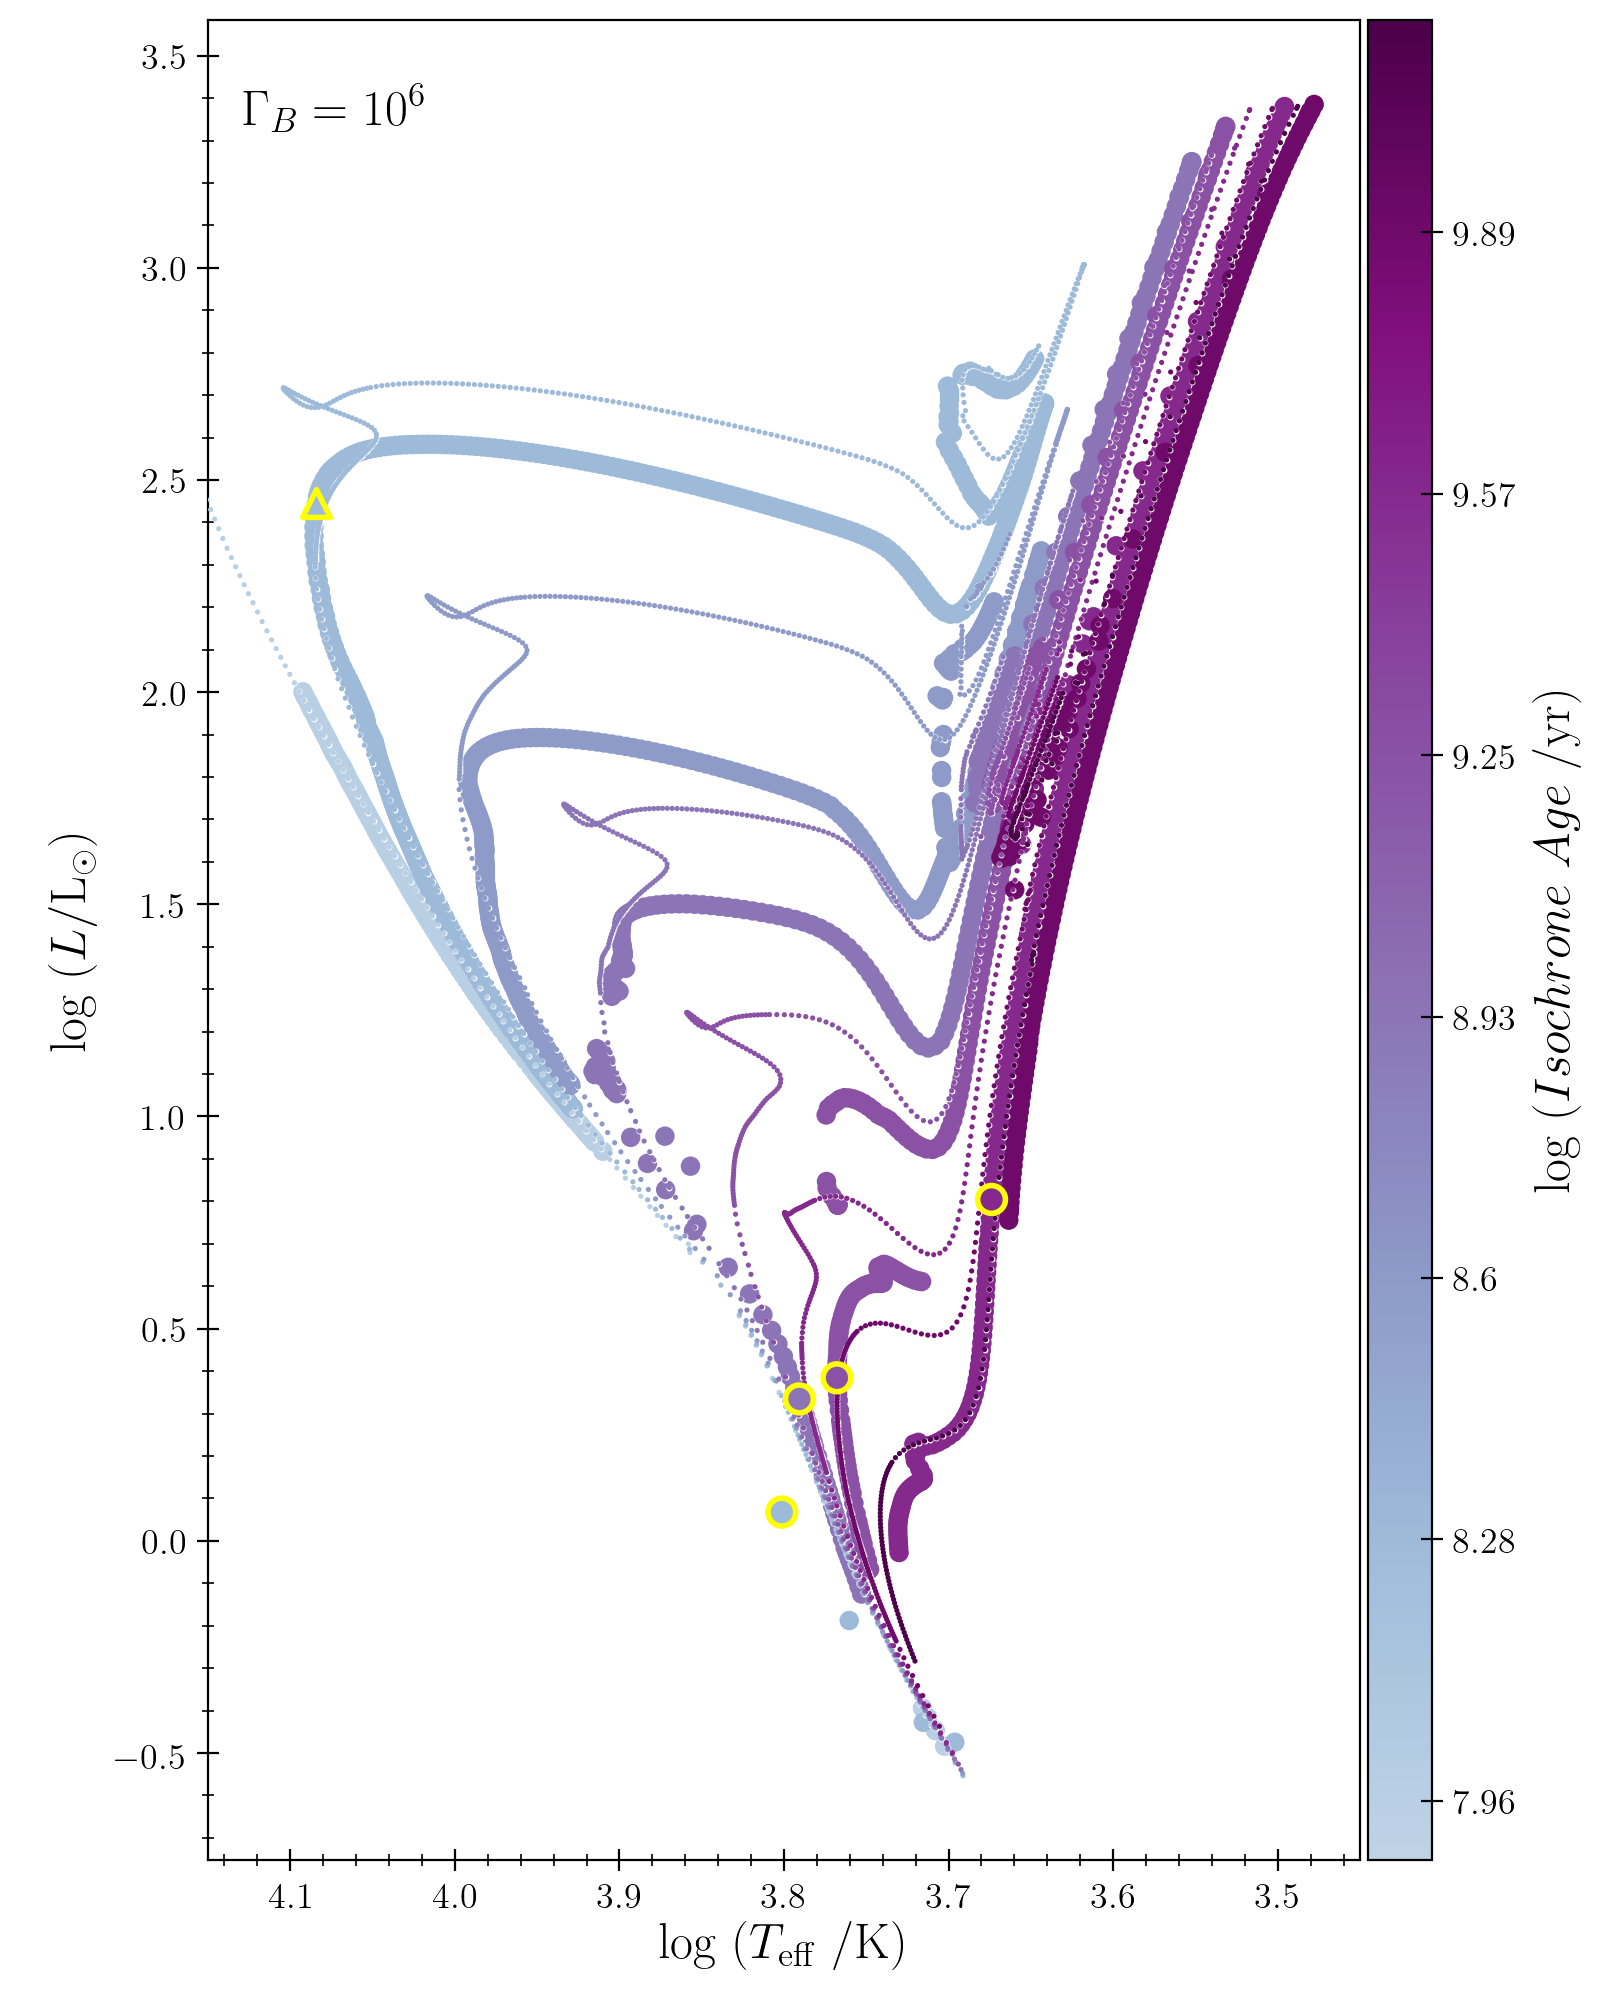
\includegraphics[width=\textwidth]{plots/isos_cb6.png}
    \caption{Same as Fig.~\ref{fig:isos_cb4} but for $\gbpow{6}$. Note
    \nodm models are overplotted as thin lines. Triangles mark $3.5 \Msun$, circles mark $1.0 \Msun$. The oldest isochrone does not appear here since all stars in our mass range that live in $\gbpow{6}$ environments evolve beyond the thermal pulse before this time. Note also that the second oldest isochrone (the oldest appearing here) does not include any stars with $\Mstar \ge 1.0 \Msun$ for the same reason.
    % Note the differences in the number and positions of these markers relative to Fig.~\ref{fig:isos_cb4}.
    }
    \label{fig:isos_cb6}
  \end{figure*}


  % hottest MS Teff plots
  \begin{figure*}
    \centering
    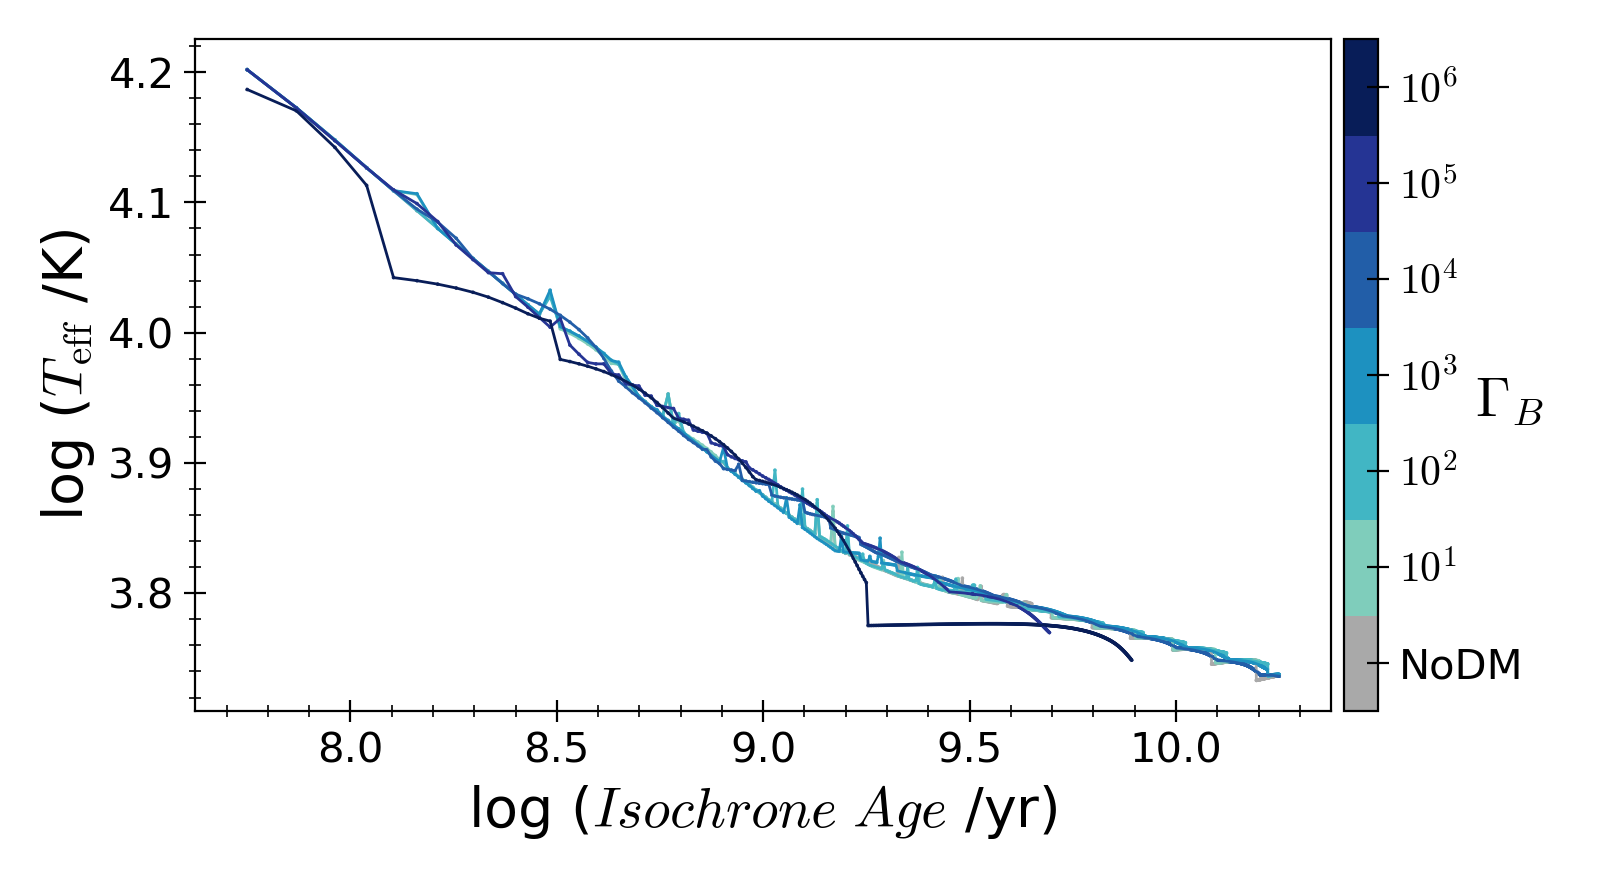
\includegraphics[width=\textwidth]{plots/hotTeff.png}
    \caption{
    Temperature of the hottest MS star. Models with $\gbpow{5}$ and $\gbpow{6}$ show significant decreases in $\Teff$ as higher mass stars leave the MS earlier than in \nodm models, leaving only cooler low mass stars.
    }
    \label{fig:hotTeff}

  \end{figure*}

    \begin{figure*}
    \centering
    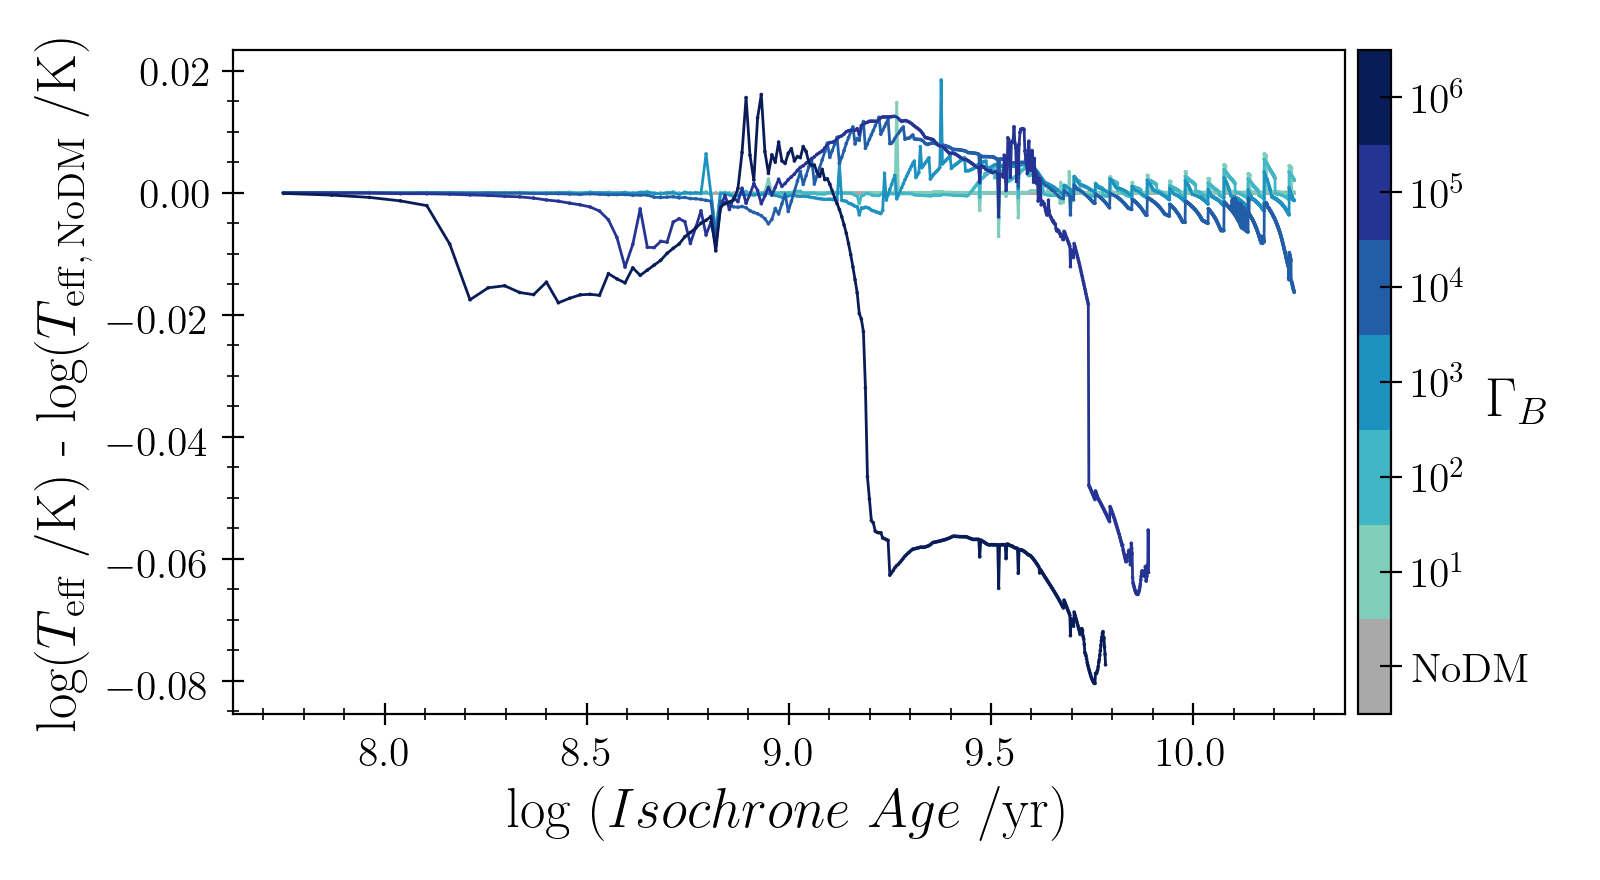
\includegraphics[width=\textwidth]{plots/hotTeff_resid.png}
    \caption{
    Residuals of previous (should do one or the other, or combine the plots. Wanted to see what Carlos says before proceeding.)
    }
    \label{fig:hotTeff}

  \end{figure*}


%   \todo{still need to re-write this paragraph.} We find that, for stars significantly affected by ADM energy transport, the general effect is to shorten MS lifetimes (see Figure \ref{fig:mstau}) so that, for a stellar populations of a given age, the MS turn-off happens at a lower mass and the stars evolve through the sub-giant branch at a lower luminosity (see Figure \ref{fig:isos}) when ADM cooling is operative. This causes isochrones of clusters in high $\gb$ environments to appear older than their standard model counterparts. This becomes noticeable in the highest $\gb$ environments around 0.2 Gyr as stars with $\rm{M} \approx 4 \Msun$ begin to leave the MS. Prior to this the stars have not had enough time to capture a sufficient number of WIMPs for ADM-driven energy transport to be a significant contribution to the overall energy transfer within the star.

%   \arz{In what follows, an important change will be that we should discuss the figures in the order in which they appear.
%   This is very standard practice and I don't think we should deviate from that.}

%   \arz{For this first paragraph, I might attempt to do something like the following. I think this
%   gives a nice introduction to the basic result, incorporates what the reader needs to know about
%   low-and high-mass stars (so we can remove that part from the introduction), and segues into
%   the separate subsections about low- and high-mass stars. This may need some editing, but I hope
%   you get the idea.}

  In general, we find that ADM captured by stars alters main sequence lifetimes, as seen in Figs.~\ref{fig:mstau} and ~\ref{fig:Teff}.
  For the purposes of Fig.~\ref{fig:mstau} we have defined the
  MS to end when the fractional abundance of hydrogen in the core, $X_c$, falls below $10^{-3}$. $X_c$ declines rapidly at the end of the MS, so our results are not strongly affected by the exact choice.
  Fig.~\ref{fig:Teff} illustrates the effect for select $\gb$ on the stellar surface observable $\Teff$.

  In Fig.~\ref{fig:mstau},
  it is apparent that in most, but not all, scenarios that we study, MS lifetimes are reduced due to ADM.
  Examining Fig.~\ref{fig:mstau} more closely, stellar lifetimes relative to the standard case with no
  ADM increase from low masses until they turn over and decrease again. The mass at which this decrease
  occurs varies based upon the environmental boost factor, $\gb$, which is a proxy for the strength of the
  cooling effect. However, the reason for the turnover is related to a fundamental distinction between
  low-mass stars and high-mass stars. \qus{Andrew, I think you wrote this part... isn't the relevant turnover from decreased lifetimes back to no change in lifetimes, rather than from increasing to decreasing lifetimes?} \tjh{I think we should comment a little more on the stars who have their MS lifetimes prolonged. I think this is just due to the core being cooled, so fuel is burned through at a lower rate. Also, would it be correct to say that large amounts of ADM shift the distinction between low-mass and high-mass stars to higher masses? And that low-mass stars have their lifetimes prolonged.}

  To understand this feature better, consider standard stellar evolution in which there is no influence from
  dark matter of any kind. In this case, stars burn hydrogen to produce helium through two channels, namely
  the proton-proton (pp) chain and the carbon-nitrogen-oxygen (CNO) cycle
  \arz{Cite one or more standard references on stellar structure here. I am partially
  to Kippenhahn, but whatever you like is fine.}. The pp chain dominates energy
  production in stars with core temperatures $\Tc \lesssim 2 \times 10^7 \K$ and the
  rate of burning scales with temperature very roughly as $\epspp \propto T^4$. The CNO
  cycle dominates nuclear burning in stars with higher core temperatures and CNO burning rates scale
  much more strongly with temperature: $\epsCNO \propto T^{16-20}$. The core temperature
  that separates the CNO cycle from the pp chain corresponds to a stellar mass of approximately
  $\Mstar \sim 1.3 \Msun$. This distinction in burning rates causes a fundamental
  difference in stellar structure. In pp-dominated stars ($\Mstar \lesssim 1.3 \Msun$),
  the transport of energy from the core burning region
  is dominated by photon diffusion. Energy transport in the cores of such stars
  is said to be radiative. In CNO-dominated stars ($\Mstar \gtrsim 1.3 \Msun$),
  radiative energy transport is insufficient to carry away the energy produced by hydrogen burning.
  Consequently, these high-mass stars have convective cores. In \S~\ref{sub:highmass} and \S~\ref{sub:lowmass}, we will consider
  results for high-mass stars and low-mass stars separately and we will demonstrate that ADM
  has distinct effects on the evolution of the two groups.

  The effects of ADM on a single star's evolutionary track in an HR diagram (Fig.~\ref{fig:tracks}) are generally subtle since the most significant effect on the stellar surface properties $L$ and $\Teff$ is to move the star through roughly the same sequence of events at a more rapid pace. The location of the ZAMS is set by the balance between pressure support from nuclear burning and gravitational contraction, which depends only on the mass. The temperature of the red giant branch is set by an equilibrium between neutral and ionized hydrogen in the atmosphere. Hence, the star's HR track cannot be too different from the \nodm models.

  The change in the evolution to do ADM is more obvious in the isochrones of stellar populations, since the time dependence is explicit here. Populations in high $\gb$ environments appear older than their \nodm counterparts (Fig.~\ref{fig:isos_cb4} and Fig.~\ref{fig:isos_cb6}). \todo{explain the gaps due to failure of interpolation in these plots.} \qus{How can the true age of a stellar population be determined/estimated so that observations can distinguish between old populations in \nodm environments and younger ones in high $\gb$ environments?}

\subsection{High-Mass Stars: \mrangehigh}
\label{sub:highmass}

  % 3.5Msun, energy and convection
  \begin{figure}
    \centering
    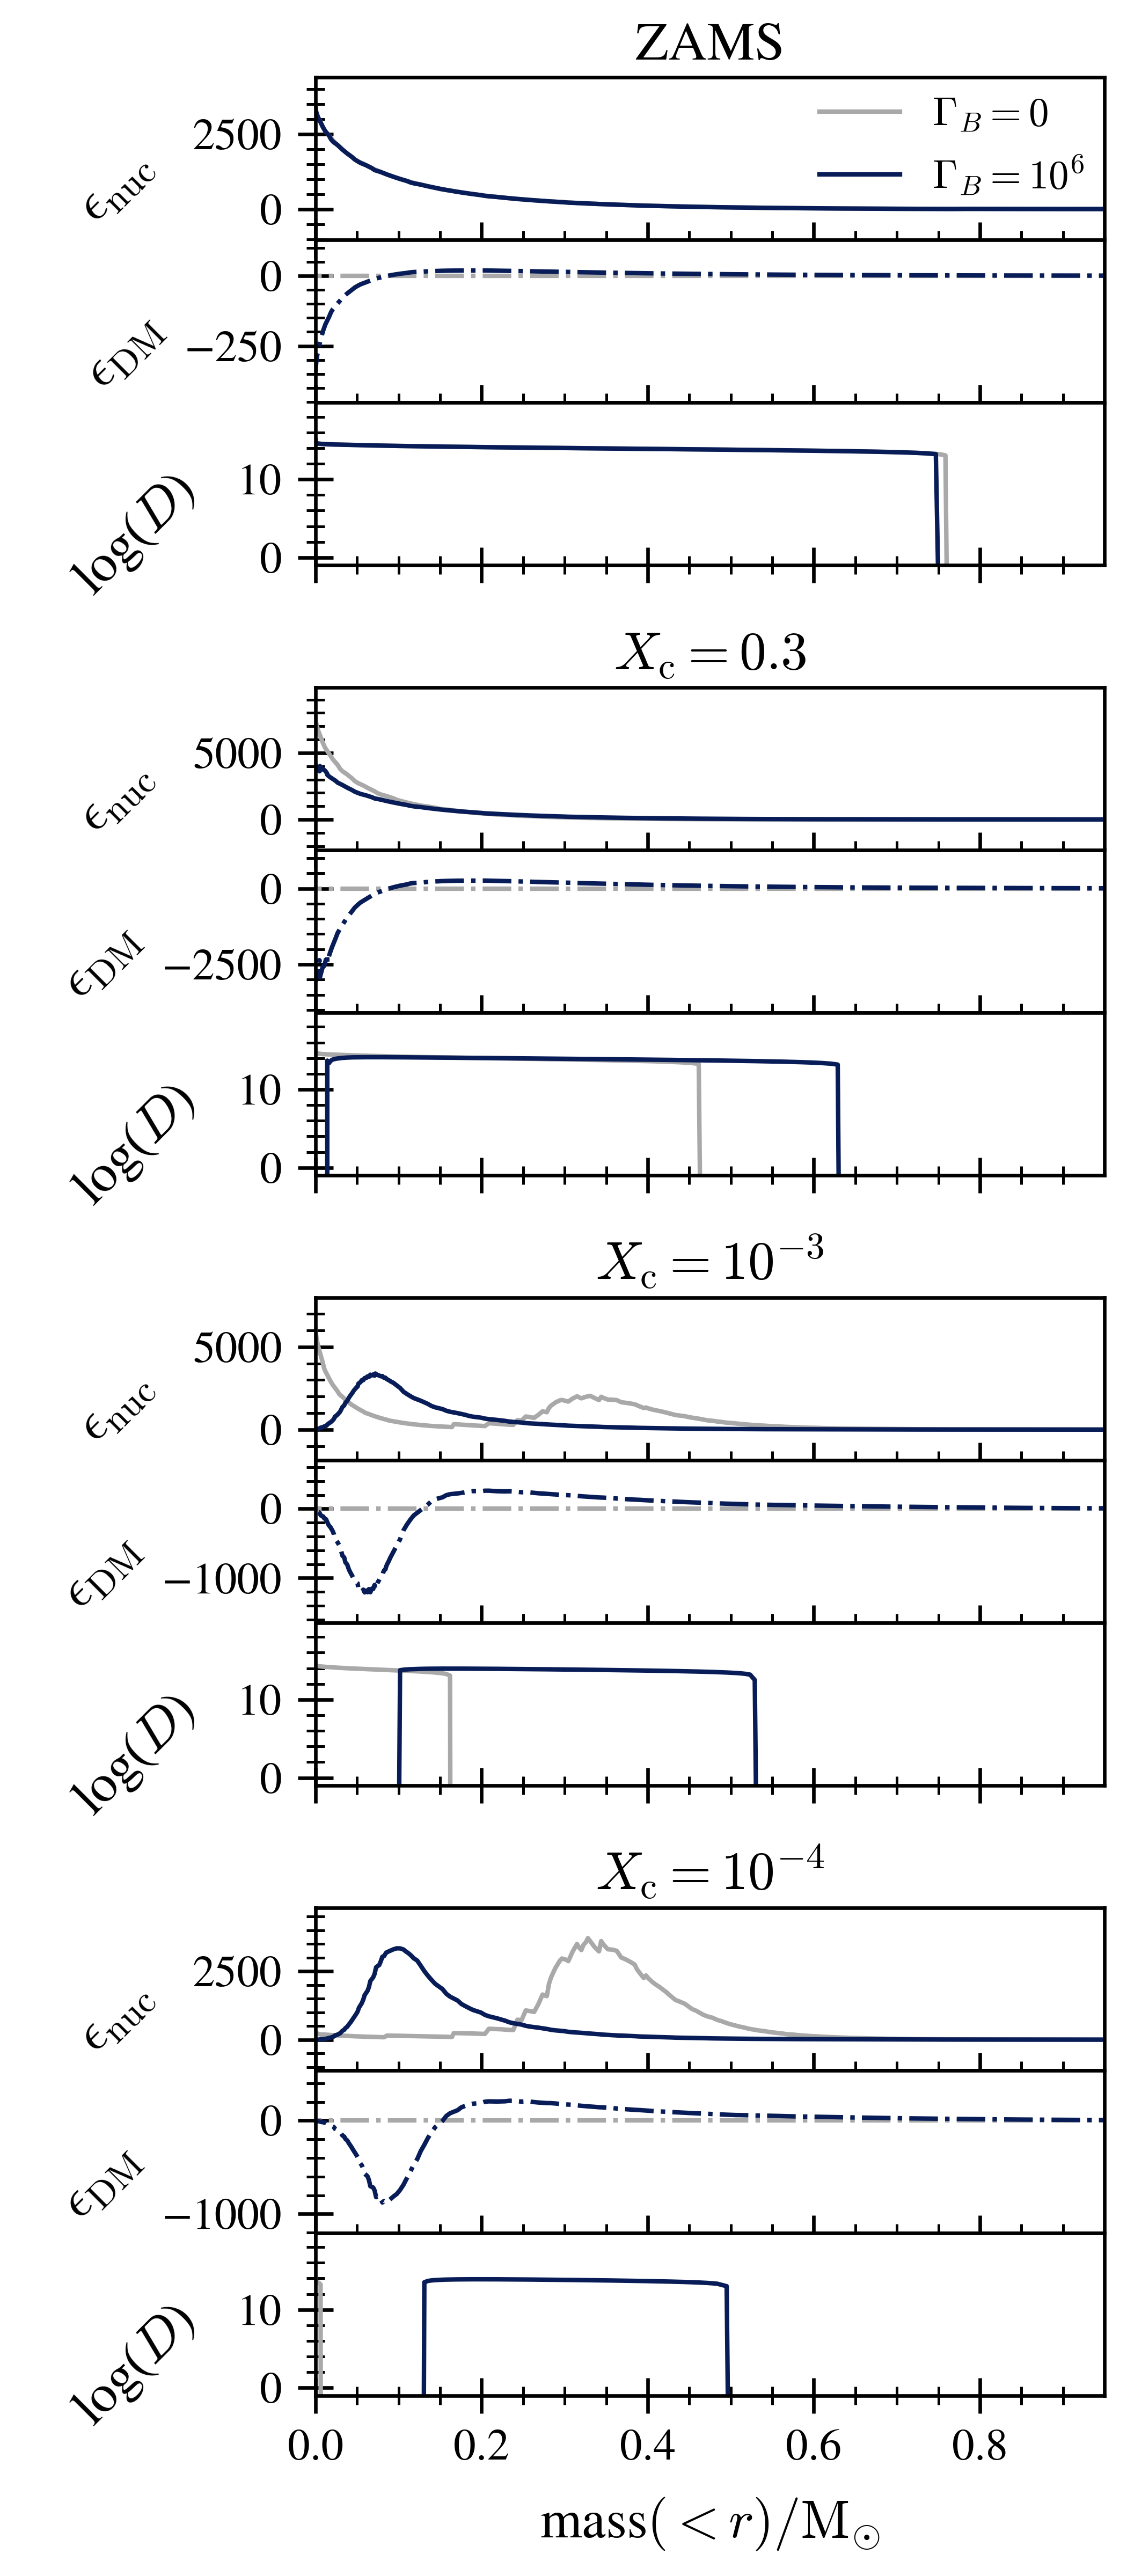
\includegraphics[width=0.47\textwidth]{plots/m3p5.png}
    \caption{$3.5 \Msun$ profiles for \nodm (grey) and $\gbpow{6}$ (dark blue) models. Each set of 3 panels shows: 1) nuclear burning rate in [erg/g/s], 2) rate of energy transport by ADM, also in [erg/g/s], 3) the diffusion coefficient for convective + overshoot mixing in [cm$^2$/s]. Time moves down the page. As the radiative core grows in the $\gbpow{6}$ model, the burning shifts outward into a shell, following the inner edge of the convective zone. The hydrogen supply is not replenished outside the convective zone, resulting in $\gbpow{6}$ models leaving the main sequence earlier due to core hydrogen depletion.
    }
    \label{fig:m3p5}
  \end{figure}

  In standard models, MS stars with $\Mstar \gtrsim 1.3 \Msun$ are powered primarily by the CNO cycle.
  This has several important consequences:
  (1) the burning rate is much higher than in pp-dominated stars;
  (2) the burning rate is extremely sensitive to core temperature;
  and (3) stellar cores must be convective in order to carry away the
  energy produced by core hydrogen burning.
  Central convection extends beyond the burning region,
  giving the star a source of fresh nuclear fuel as hydrogen from outside of the
  core is mixed into the center.
  This influx of unburnt hydrogen extends the MS lifetime of the star beyond what it would have been without convection.
%   \footnote{This extension is subdominant. Central temperatures increase with stellar mass, causing the burning rates to increase dramatically which shortens standard model stellar lifetimes so they decrease approximately as $\tau \propto \Mstar^{-2.5}$.}.
  Once hydrogen throughout the convective zone is depleted, the burning rate rapidly decreases, and
  the star loses more energy at its surface than is being generated by burning.
  Gravity temporarily dominates and the star contracts until the
  internal temperature increase is sufficient to ignite hydrogen in a shell
  outside the depleted core.
  This can be seen in the bottom panel of Figure~\ref{fig:m3p5} where the `\nodm' (light green) burning rate has significantly decreased at the center and increased at $m(<r) \sim 0.4 \Msun$ in the relatively short time since the panel above it.
%   \qus{why does the convective region shrink while burning rate increases?}
  The contraction causes a temporary increase in
  $\Teff$ and a feature in the star's HR diagram called the convective hook (see Figures \ref{fig:tracks} and \ref{fig:isos_cb}). \qus{Maybe I should leave this last sentence out? I may be overemphasizing the convective hook here and in what follows.}
  See \citet{Pols1990StellarEvolution} for more details.
%   \arz{If you want to discuss Figure~5 prior to discussing the isochrones,
%   then we should switch the order in which the
%   figures appear in the paper. Figure~5 will
%   need a detailed caption and/or a more detailed description
%   in the main text of the paper.}


  If a star captures enough ADM, the combination of dark matter + radiative energy transport becomes sufficient to carry the flux from nuclear burning. Convection disappears from the center first (where ADM energy transport is most efficient) and retreats away from the core, into a narrowing shell. Without convective mixing, the central hydrogen supply depletes and the burning also shifts into a shell, following the lower boundary of the convective zone. This can be seen in the time progression (down the page) of the $\gbpow{6}$ (dark blue) model in Figure~\ref{fig:m3p5}. The result is that these stars leave the MS earlier and at a lower luminosity, and they skip the convective hook altogether (Figure \ref{fig:tracks}). This makes the isochrones appear older than their `\nodm' counterparts (Figure \ref{fig:isos_cb}). \tjr{I know I need to explain these 2 figures a little more. I'll update the plots and write better captions and then see what else I need to say here.} The effects disappear as $\Mstar$ approaches $5 \Msun$ because stellar lifetimes become too short for a sufficient amount of ADM to build up.


\subsection{Low-Mass Stars: \mrangelow}
\label{sub:lowmass}

  % 1.0Msun, energy and temperature
%   \begin{figure}
%     \centering
%     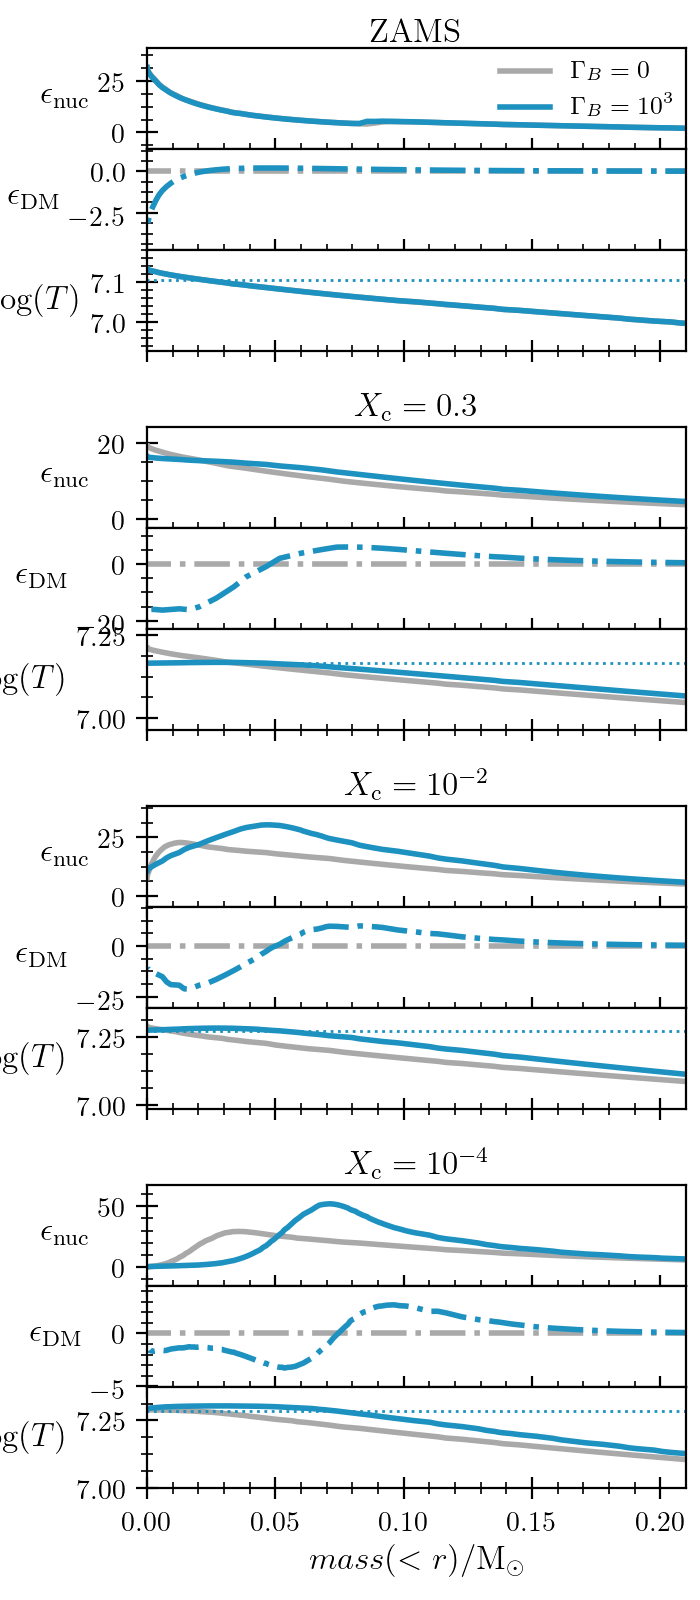
\includegraphics[width=0.47\textwidth]{plots/m1p0c3.png}
%     \caption{$1.0 \Msun$ profiles for \nodm (grey) and $\gbpow{3}$ (blue) models. In each set of 3 panels, the top 2 are the same as in Figure~\ref{fig:m3p5}. The third panel is the temperature in [K], with the characteristic ADM temperature, $\Tx$, shown as a thin dotted line. ADM energy transport decreases hydrogen burning in the core and pushes the burning into a shell more quickly than the reference models. The reduced central burning causes the $\gbpow{3}$ model to live slightly longer than the \nodm model.
%     }
%     \label{fig:m1p0_a}
%   \end{figure}

%   % 1.0Msun, energy, temperature, density profiles
%   \begin{figure*}
%     \centering
%     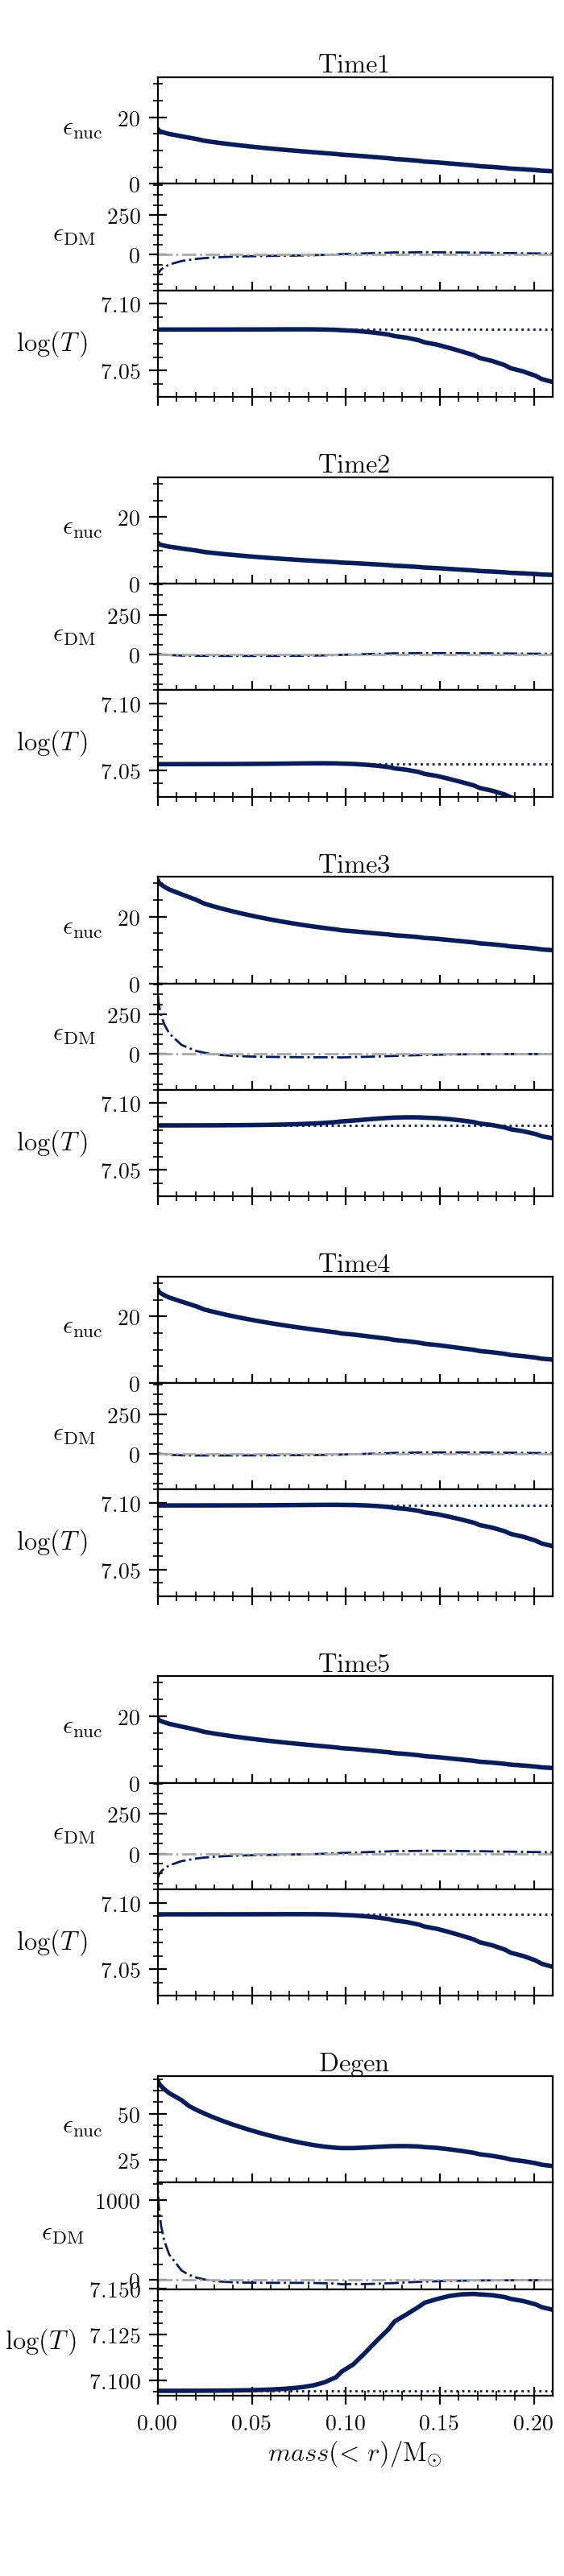
\includegraphics[width=\textwidth]{plots/m1p0c6.png}
%     \caption{$1.0 \Msun$, $\gbpow{6}$ profiles. Time moves down the page (rows correspond to times noted in Fig.~\ref{fig:m1p0_kipp}) and were chosen to demonstrate the effects of ADM energy transport over one oscillation cycle. Scales are fixed for ease of comparison, except in the last plot where degenerate conditions cause larger changes in scale. Left column has $\epsilon_{nuc}$ on left axis (red) and DM energy transport on the right (blue). Right column has logT on left axis (red, with T$_x$ marked with thin dotted line) and logRho on the right axis (blue). \tjr{We may not need all 6 panels here. Also, I don't like that the colors here are different than anything else in the paper. Maybe it would be better to make it consistent with the previous two Figures by making all lines the same color (dark blue for $\gbpow{6}$) and make the ones associated with the right axes dotted lines.}
%     %   Time 1: 3.1736e8 yrs, xheat$_c$ is maximum, T$_c$ and $\epsilon_c$ are increasing. Time 2: 3.229e8 yrs, xheat$_c$ is minimum, T$_c$ and $\epsilon_c$ are decreasing (this should be first time shown in plot). Time 3: 3.288e8 yrs, T$_c$ is minimum, xheat$_c$ and $\epsilon_c$ are increasing. Time 4: 3.81e8 yrs, core degeneracy has become significant.
%     }
%     \label{fig:m1p0_profs}
%   \end{figure*}

  % 1.0Msun c6 Kippenhahn with profile times labeled
  \begin{figure*}
    \centering
    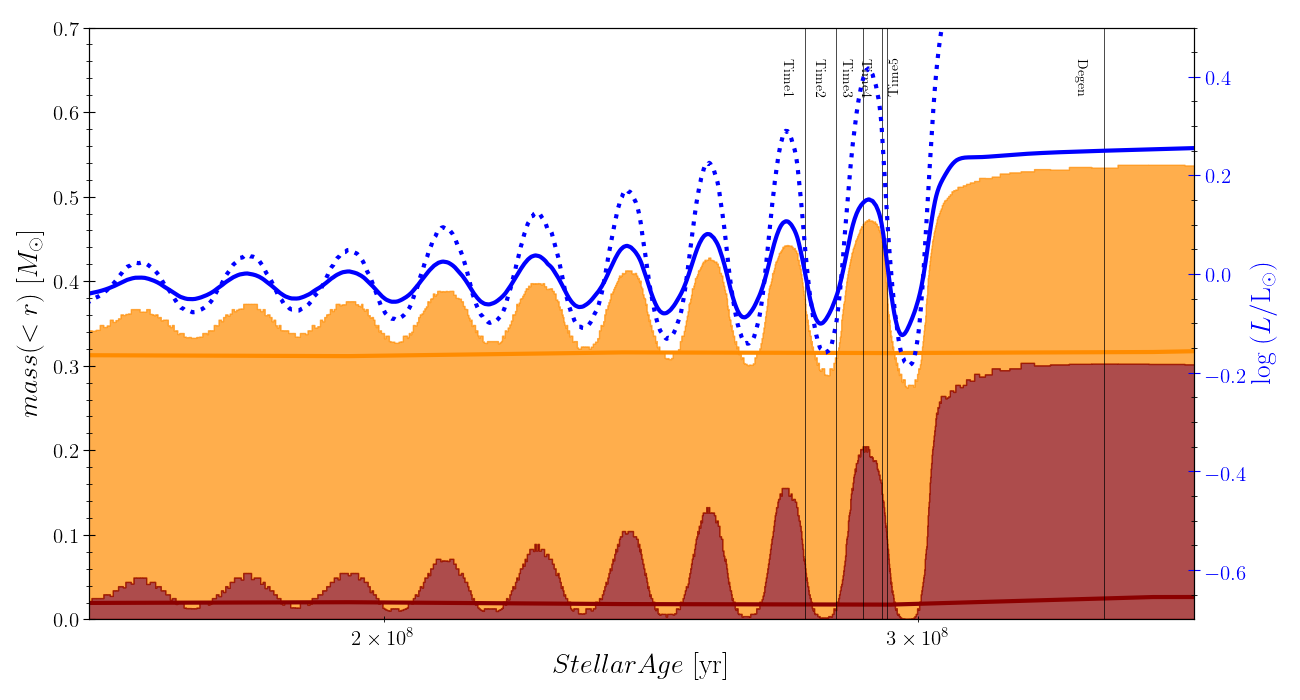
\includegraphics[width=\textwidth]{plots/m1p0c6_kipp.png}
    \caption{Time evolution of a $1.0 \Msun$, $\gbpow{6}$ star.
    % Star mass 1.0Msun, c6, xaxis is age. Top plot shows core burning volume (red shaded area, left axis. Add color variations to show intensity) and L (right axis. Important lines are in the middle, red (log L) and white (log LH). Top and bottom lines should be removed from plot.
    Yellow and red shaded regions show burning intensity as a function of the mass coordinate (left axis). Yellow indicates (I believe the burning thresholds are 1 erg/g/s and 10 erg/g/s respectively, but I'm a little confused about the mesa output and I need to check with Héctor or Carles.) Darker yellow and red lines mark the burning extent of the \nodm model over this time period.
    Blue line is luminosity (right axis).  Fig.~\ref{fig:m1p0_profs} shows profiles of the star at the times marked here by vertical black lines.
    \tjr{Dotted blue line is hydrogen burning luminosity. I will probably remove this line for the final plot, but I want to check with Carles to make sure the behavior makes sense. I think the explanation is: When LH>L star is producing more energy than it is losing, causing it to expand, but I'm not sure why we don't have LH = L after degeneracy. I have a separate plot of the radius that we can look at if needed. (Actually could add logR to this plot.)}
    %   (bottom plot). Bottom plot shows R$_{\star}$ (yellow, left axis) and r(m<0.01). As the core contracts, the envelope expands.
    }
    \label{fig:m1p0_kipp}
  \end{figure*}

  Standard model stars in this mass range have relatively low central temperatures and so are powered primarily by the pp chain, which is much less sensitive to the temperature. This means the burning does not peak as strongly at the center and radiative transport is sufficient to carry the energy flux, so the core is not convective. Without convective mixing, hydrogen depletes first at the very center and the burning shifts outward gradually, avoiding the instability that causes the convective hook in standard CNO-powered stars. This behavior is very similar to high-mass stars that collect large amounts of ADM, which contributes to isochrones appearing older as $\gb$ gets large.

  Since the burning rate is much lower, the same number of captured dark matter particles have a larger effect in this mass range. As stars with $\gb$ as low as $10^2$ \todo{check this number for several masses} enter the MS, ADM is already transporting a significant amount of energy away from the center ($\epsx \approx \epspp$ near $r=0$) and depositing it in a shell at $m(<r) \approx 0.1 \Msun$. This causes the temperature, and therefore the burning rate, to be lower at the center and higher in a shell relative to standard models. Stars in environments with $\gb \lesssim 10^4$ are able to remain stable in this configuration. See Figure~\ref{fig:m1p0_a}.
  % and their evolution is not significantly altered \tjr{looks significant in MStau plot...?}.

  Models with $\gb \gtrsim 10^4$ capture enough ADM so that $\epsx \gg \epspp$ near $r=0$ which destabilizes the core and sets up a series of oscillations which are shown in Figure~\ref{fig:m1p0_profs}. \todo{check different masses, particularly 0.8Msun for which the effect may extend down to c4.}
 As $\Tc$ continues to decrease, the temperature profile inverts and the center is no longer the hottest region in the star. Eventually, $\Tc < \Tx$ and dark matter begins moving energy back towards the center ($\epsx(r=0) > 0$, see Time 3 in Figure \ref{fig:m1p0_profs} \todo{possibly pick this time a little later, after xheat at center >0}). This increases both the central temperature and burning rate until $\Tc > \Tx$ and the cycle starts over. The effects propagate out to the surface where
  $L$, $\Teff$, and $\Rstar$ all oscillate in response to changes in the core (Figure~\ref{fig:m1p0_kipp}). Similar oscillatory behavior was noted in \citet{Iocco2012} \qus{seems like I need to say more here, but I'm not sure what. The Iocco paper (arXiv:1201.5387v1) states the following: "In spite of our efforts, we have not been able to fully understand the reason of the oscillations seen in Figure 3, whether they are a physical effect arising from the “bouncing” of the central temperature on the WIMP temperature floor, or a numerical artifact. We have however checked that the existence of oscillations does not affect our results nor does change our conclusions. Beside the theoretical consistency of the intepretation presented in the paper, one can be convinced of the actual physical consistency of our results with observations based on several numerical experiments we have performed: ..."}.

  The process repeats, with increasing amplitude, until the central temperature falls low enough that the core becomes significantly degenerate. Once electron degeneracy pressure can support the core, the temperature decouples from the equation of state and the star quickly settles into a more stable configuration with a significant temperature inversion (see Time 4 in Figures \ref{fig:m1p0_profs} and \ref{fig:m1p0_kipp}).

  Overall, the ADM captured by these stars causes burning in a larger volume and at a higher rate than in standard models (see Figure \ref{fig:m1p0_kipp}). The stars then burn through the central hydrogen supply faster and leave the MS earlier: by 2.5 Gyr, solar mass stars with $\gbpow{6}$ have already left the MS and are climbing the red-giant branch. Note that the 2.5 Gyr, $\gbpow{6}$ isochrone is most similar the 10 Gyr, \nodm isochrone in Figure~\ref{fig:isos_cb}.


  Notes:
  hydrogen depletes in shell first.
  % \tjr{I'm not totally sure this is the CAUSE of the oscillations, but I've checked a lot of other things and ruled them out. Lower cboost models sometimes transport more energy than produced by burning, but never more than a few erg/g/s. c5 and c6 models transport a minimum of ~5 erg/g/s more than is generated from burning and usually much more than that (a few hundred erg/g/s during oscillations, up to 1000 erg/g/s by the time it goes degenerate).}

  % \tjr{burning changes before temperature which I don't really understand. See figure \ref{fig:osc_scaled_values} for more info. Order of changes seems to be: extra heat -> density -> burning -> temperature. Tried to check how mesa calculates the burning rate to find dependencies other than temperature, but the calculation seems pretty scattered and complicated and I couldn't find anything useful.}

% fe Pre-Sprint Results Section
